% ============================================================
%  第十一章 强关联电子体系（前半：§1–§6）
%  底本：高等教育出版社《固体理论》第二版；原书印刷页 390–432
%  （PDF 页 = 印刷页 + 20；§1 约印 390–402，§2 约印 402–411，
%   §3 印 411–415，§4 印 415–417，§5 印 417–426，§6 印 426–432）
%  后半 §7–§11 及章末参考文献见 ch11b.tex（原书第十一章文献在
%  §11 之后，印刷页 456 起）。
%  公式编号自检：§1 (11.1.1)–(11.1.65)；§2 (11.2.1)–(11.2.42)；
%    §3 (11.3.1)–(11.3.26)；§4 (11.4.1)–(11.4.13)；
%    §5 (11.5.1)–(11.5.42)；§6 (11.6.1)–(11.6.21)
%    （(11.6.6a/b)、(11.6.9a/b) 为原书自带二级编号，用
%    subequations 环境照录，与 ch04/ch06 体例一致）。
%    全半区自动编号 209 个，无缺号。
%
%  任务单所列 ch11 "缺号"（本半区相关者）逐条对照原书页面判定，
%  均非原书跳号，系 OCR 把 (11.x.y) 误作 (1.x.y)（少首位 1）或
%  编号碎裂，已按页面归还：
%    (11.1.38) tag 作 (1.1.38)（p395 在号）；
%    (11.1.45) 编号碎裂嵌于式内（p397），已归还；
%    (11.1.64) 编号以散字"(11.1.64)"混入式尾（p400），已归还；
%    (11.2.21) tag 作 (1.2.21)（p406 在号）；
%    (11.2.24) OCR 将 (11.2.23)/(11.2.24) 并成一块、只剩游离
%              "(11.2.24)"文字——原书 p406 为 ω±iη 两个独立编号
%              公式，已按页面拆为两式；
%    (11.2.26) 谱定理式编号碎裂（p407），已复原；
%    (11.2.27) tag 残作 (.27)（p407 在号），已归还；
%    (11.3.1)  tag 作 (1.3.1)（p412 在号）；
%    (11.3.12) tag 残作 (.12)（p413 在号），已归还；
%    (11.3.21) tag 残作 (21)（p414 在号），已归还；
%    (11.3.22) 编号碎裂（p415），已归还；
%    (11.4.4)  tag 作 (1.4.4)（p416 在号）；
%    (11.5.1)  编号碎裂混入正文（p417 在号），已排为编号公式；
%    (11.5.11) 编号碎裂（p420 在号），已归还；
%    (11.6.6)(11.6.9) 原书即分 a/b（p428、429），照录。
%    （任务单另一批"1.1/1.2/1.4/1.11 缺号"实为 (11.x.y) 之
%    OCR 误读，不属于本半区问题。）
%
%  已修正的 OCR/原书错误（除全角句点转"."、删 ~ 间隔符、收紧
%  \mathrm{d}、拆开行内公式与中文、函数名复原等常规项外）：
%  1. (11.1.2) 求和指标与算符按 p391 复原为 k₁,k₂,k'₁,k'₂ 及
%     C⁺_{k₁σ}C⁺_{k₂σ'}C_{k'₂σ'}C_{k'₁σ}（OCR 指标重复、"C⁻"
%     乱码）；(11.1.1) 两行原书一个编号，已合并。
%  2. (11.1.10)(11.1.13)(11.1.15) 中 n_{iσ}n_{iσ̄} 等按 p392 复原
%     （OCR 丢 σ̄ 杠）；(11.1.11) σ=↑,↓。
%  3. §1.1 末段 OCR"！T₁1正比于""ΔĒ比于""T₀\Δ"乱码，按 p392–393
%     复原为"不难证明|T₁|正比于…""宽度Δ正比于|T₁|""T₀、Δ（或
%     T₁）和U…其中T₁<0."。
%  4. (11.1.19) Z_G、T_r、ℋ=H−μN 按 p393 复原（OCR "≤X>、Z_6"
%     乱码）。
%  5. §1.2 正文 OCR"当它位于μ能带之中时"衍字符 μ，按 p394 删
%     （原书"当它位于能带之中时"）。
%  6. (11.1.23) 式尾杂符"(i)"已删（p394）。
%  7. (11.1.32)–(11.1.37) A=n_{iσ̄}C_{iσ}、n²_{iσ̄}=n_{iσ̄}、
%     <n_{iσ̄}> 及 δ_{ij} 按 p395 复原（OCR 的 S_{ij}、σ/σ̄ 混乱
%     等均已清）。
%  8. (11.1.41) 第四项带波浪号的算符 C⁺_{iσ̄}C_{lσ̄}−C⁺_{lσ̄}C_{iσ̄}
%     及正文对应平均值 (<C⁺_{iσ̄}C_{lσ̄}>−<C⁺_{lσ̄}C_{iσ̄}>) 按
%     p397 复原；式内波浪着重线未排（见遗留问题）。
%  9. (11.1.53)(11.1.56) 按 p398–399 复原为 E^(1)/E^(2)、
%     A^(1)/A^(2) 并列两支解（OCR 只剩残行、√ 内乱码）；
%     (11.1.55) 首行 A^{(i)}_{kσ}=∂E^{(i)}_{kσ}/∂E_k。
% 10. (11.1.57) 第二行按 p399 复原为 (i/2πN)Σ_k{G_k^σ(ω+iη)−
%     G_k^σ(ω−iη)}(η=+0)（OCR 严重乱码）。
% 11. §1.5 "(Δ/U)_c"之 OCR 上标 † 经 300dpi 放大核对为印刷噪声，
%     已删（p401）。
% 12. §2.1 V_kd 第二等式、"ℋ是单电子哈密顿量"补 ℋ；朗德因子
%     "g₀=g_i=2"按 p404 复原（OCR "θ0 σ=σ_{g_i}" 乱码）。
% 13. (11.2.8) 末项原书衍一"["，按第二套运动方程通式(11.2.11)
%     更正为 <<A(t);[B,H]>>（p405）。
% 14. (11.2.13)(11.2.16)(11.2.17)(11.2.20)(11.2.23)(11.2.24) 中
%     n_{dσ̄}、Ẽ_{dσ} 等上下标按 p405–406 复原；(11.2.18) 线性化
%     近似式按 p406 复原（OCR n_{dσ}n_{dσ}）。
% 15. p408"利用态密可以计算"→"利用态密度可以计算"（原书漏字，
%     补"度"）。
% 16. (11.2.45) "和 Γ/U={…}"之"和"按 p430 复原（OCR 作花体 ℋ）。
% 17. §2.4 图 11.7 图注 OCR 粘进行文（"当图 11.7 安德逊哈特利-
%     福克解的…区域"），按 p411 拆出图注，"当"字归回正文；
%     "周期性定德逊模型"→"周期性安德逊模型"（p411）。
% 18. (11.3.3) 按 p412 复原（OCR 引号/箭头乱码）；(11.3.8) 算符
%     上下标经 300dpi 放大核对复原为 C⁺_{kσ}C_{k'σ}C⁺_{nσ'}C_{nσ'}
%     与 C⁺_{kσ}C_{k'σ'}C⁺_{nσ'}C_{nσ}（p413）。
% 19. 原书 p413 "将交换项式(11.3.9)改写成"引号有误：交换项定义
%     于式(11.3.10)，已更正。
% 20. (11.3.11)(11.3.12) 两块严重乱码按 p413 重排复原；
%     (11.3.21)(11.3.22) 按 p414–415 复原（OCR 算符残缺）。
% 21. 原书 p415 "可将 s-d 互作用式(11.3.11)改写成"引号有误：
%     所改写的是已代入 J、U 的(11.3.21)，已更正。
% 22. 原书 p415 (11.3.25) 末算符印作 C⁺_{kμ}C⁺_{k'μ'}，第二个
%     上标 + 为衍符，按 (11.3.22) 更正为 C⁺_{kμ}C_{k'μ'}。
% 23. (11.4.11) 主值积分花体 𝒫 按 p417 复原（OCR 作 𝓡）。
% 24. 原书 p419 (11.5.10) 前因子印作 (J/S)²，按 (11.5.9) 更正为
%     (J/N)²（量纲与同式结构）。
% 25. (11.5.13)(11.5.14)(11.5.25)(11.5.32) 等 cases 中文条件
%     "（当…时）"按 p420、424、425 复原（OCR 乱码）。
% 26. (11.5.19)(11.5.20) 熵花体 𝒮 统一 \mathscr{S}；(11.5.21)
%     三式合排，χ_杂质、c_杂质 等中文下标以 \text{} 照排。
% 27. (11.5.35) "ΣΓ_k=常数"按 p425 复原（OCR "‡‡𝒳" 乱码）；
%     (11.5.40) 复原为 exp[−2/(|J|ρ_F)]（p425）。
% 28. 原书 p426 "必须同时考虑所有粒子相互用的真正多体问题"
%     漏字，补"作"作"相互作用"；原书 p422 "(贝本章§9)"为
%     "见"之误（与并行句"(见本章§10)"一致），已更正。
% 29. §5.3 末段 OCR "U>>T"→U>>Γ（Γ 为 (11.2.22) 定义的线宽，
%     p432）；"钢系"→"锕系"；"有效质量的m_e下界"衍 m_e 已删
%     （p452"有效质量的下界"）。
% 30. 原书 p428 "施里弗-沃尔夫变则只是在"漏字，补"换"作
%     "变换则只是"。
% 31. (11.6.9a)(11.6.9b) 按 p428–429 复原（OCR tag 残作"9b"）；
%     (11.6.11)(11.6.12) 按 p429 重排（OCR 的 C_{k't'} 类乱码
%     复原为 ↑/↓ 自旋指标）。
% 32. 原书 p430 (11.6.19) 首项印作 Ŝ（无上标），按 (11.6.16)
%     补 Ŝ^z；该式 OCR 严重乱码已按 p430 重排。
% 33. 原书 p426 §6 首句即以"讲的是如何…"起（承章题省略主语），
%     照录未改（见遗留问题）。
%  插图：图 11.1–图 11.14 共 14 幅（任务单所称"本半区含
%  图11.1–图11.7"有遗漏——图 11.8–图 11.14 亦在 §5–§6 区间内，
%  均已按原书页面排出）。
%  遗留问题：
%  · 图 11.1–11.14 均为占位图（figures/fig11-N.pdf），待重绘代理
%    按原书绘制；
%  · (11.1.41) 原书在带波浪号的算符部分下有"~~~"着重线，本稿
%    未排波浪线，仅以正文"有"~~~"号的算符部分"照录；
%  · §6 首句"讲的是如何从安德逊模型导出 s-d 交换模型"无主语，
%    原书如此（p426），照录；
%  · (11.1.23) 原书 δ 函数项中作 [A(t),B(t)]_+（p394），照录；
%  · (11.2.19) 第二个分母原书作 (ω−E_{k'σ})（与 (11.2.12)、
%    (11.2.15) 的同 σ 记号一致），照录。
% ============================================================
\chapter{强关联电子体系}

\section{赫伯德模型}

在小极化子理论中，我们已经看到当电子-声子互作用足够强时，离子晶体的电导不能用能带图像描述，而必须从局域模型出发建立小极化子的跳跃电导理论.这是能带论失效的一个例子，问题的关键是单电子近似忽略了电子-声子互作用对载流子状态的影响.

建立在单电子近似基础上的能带理论，不仅忽略了电子-声子互作用，而且还认为价电子在晶体中的运动是彼此独立的，因此电子间的关联作用也被忽略了.实际上在窄能带中电子间关联作用是十分重要的，因为电子从一个局域原子轨道运动到另一个原子局域轨道上时，必须考虑后一轨道是否被其它电子占据，如果已被占据，则应当计入在同一原子（或格点）周围两个电子间的库仑作用，这一作用将使能带状态发生显著的变化.

在实验上也发现，用能带论解释过渡金属化合物的特性往往是失败的.例如MnO晶体，平均每个元胞中有5个3d电子构成未填满的3d带，而O$^{2-}$的2p能带是满带，且与3d带不重叠.因此能带论说明MnO的3d带将具有金属导电性，但是测得的导电率很低，在室温下只有 $10^{-15}\,\Omega^{-1}\cdot\mathrm{cm}^{-1}$，说明MnO晶体实际上是绝缘体而不是导体，类似的情况也出现在高温超导的母体化合物如La$_{2}$CuO$_{4}$等之中.对于ReO$_{3}$，能带论预言它是绝缘体，但实际是良导体，其室温导电率为 $10^{5}\,\Omega^{-1}\cdot\mathrm{cm}^{-1}$ 与金属Cu差不多.还有些过渡金属氧化物当温度升高时会从绝缘体变为金属，这些都是能带论不能解释的.通过本节的讨论将明白，造成以上谬误的主要原因是能带论忽略了窄带中的电子强关联效应.

\subsection*{1. 赫伯德哈密顿量}

考虑N个原子组成的简单晶体，设 $h(\boldsymbol{r}_{i})$ 代表单电子在周期场中的哈密顿量，则多体系统的总哈密顿量为
\begin{equation}
\begin{aligned}
  &H=\sum_{i}h(\boldsymbol{r}_{i})
  +\frac{1}{2}\sum_{i,\,j}v_{ij}\\
  &v_{ij}=\frac{e^{2}}{|\boldsymbol{r}_{i}-\boldsymbol{r}_{j}|}
\end{aligned}
\end{equation}
为简单起见只考虑单个未填满的能带，例如孤立的s带.这时在布洛赫表象中互作用哈密顿量的二次量子化表示式可写成
\begin{equation}
  H=\sum_{k,\,\sigma}E_{k}C^{+}_{k\sigma}C_{k\sigma}
  +\frac{1}{2}\sum_{\substack{k_{1},\,k_{2},\,k'_{1},\,k'_{2}\\ \sigma,\,\sigma'}}
  \langle\,k_{1},k_{2}\mid v\mid k'_{1},k'_{2}\,\rangle\,
  C^{+}_{k_{1}\sigma}C^{+}_{k_{2}\sigma'}C_{k'_{2}\sigma'}C_{k'_{1}\sigma}
\end{equation}
其中 $E_{k}$ 是能带电子的能量，$C^{+}_{k\sigma}$ 和 $C_{k\sigma}$ 代表布洛赫轨道（k波矢）上 $\sigma$ 自旋电子的产生及消灭算符，而
\begin{equation}
  \langle\,k_{1},k_{2}\mid v\mid k'_{1},k'_{2}\,\rangle
  =e^{2}\int\frac{\psi^{*}_{k_{1}}(\boldsymbol{r})\psi^{*}_{k_{2}}(\boldsymbol{r}')
  \psi_{k'_{1}}(\boldsymbol{r})\psi_{k'_{2}}(\boldsymbol{r}')}
  {|\boldsymbol{r}-\boldsymbol{r}'|}\,\mathrm{d}\boldsymbol{r}\,\mathrm{d}\boldsymbol{r}'
\end{equation}
为了讨论窄带中关联问题，最好采用瓦尼尔表象，利用熟知的变换关系式
\begin{equation}
  \psi_{k}(\boldsymbol{r})=N^{-\frac{1}{2}}\sum_{i}
  \mathrm{e}^{\mathrm{i}\boldsymbol{k}\cdot\boldsymbol{R}_{i}}
  a(\boldsymbol{r}-\boldsymbol{R}_{i})
\end{equation}
和
\begin{equation}
\left.
\begin{aligned}
  &C^{+}_{i\sigma}=N^{-\frac{1}{2}}\sum_{k}
  \mathrm{e}^{-\mathrm{i}\boldsymbol{k}\cdot\boldsymbol{R}_{i}}C^{+}_{k\sigma}\\
  &C_{i\sigma}=N^{-\frac{1}{2}}\sum_{k}
  \mathrm{e}^{\mathrm{i}\boldsymbol{k}\cdot\boldsymbol{R}_{i}}C_{k\sigma}
\end{aligned}\right\}
\end{equation}
将式(11.1.2)变换到瓦尼尔表象
\begin{equation}
  H=\sum_{i,\,j}\sum_{\sigma}T_{ij}C^{+}_{i\sigma}C_{j\sigma}
  +\frac{1}{2}\sum_{\substack{i,\,j,\,l,\,m\\ \sigma,\,\sigma'}}
  \langle\,ij\mid v\mid lm\,\rangle\,
  C^{+}_{i\sigma}C^{+}_{j\sigma'}C_{m\sigma'}C_{l\sigma}
\end{equation}
其中 $C^{+}_{i\sigma}$ 和 $C_{i\sigma}$ 是瓦尼尔轨道（i格点）上 $\sigma$ 自旋电子的产生及消灭算符，单粒子项中
\begin{equation}
\begin{aligned}
  T_{ij}&=\int a^{*}(\boldsymbol{r}-\boldsymbol{R}_{i})h(\boldsymbol{r})
  a(\boldsymbol{r}-\boldsymbol{R}_{j})\,\mathrm{d}\boldsymbol{r}\\
  &=N^{-1}\sum_{k}\mathrm{e}^{\mathrm{i}\boldsymbol{k}\cdot(\boldsymbol{R}_{i}-\boldsymbol{R}_{j})}E_{k}
\end{aligned}
\end{equation}
互作用项中
\begin{equation}
  \langle\,ij\mid v\mid lm\,\rangle
  =e^{2}\int\frac{a^{*}(\boldsymbol{r}-\boldsymbol{R}_{i})
  a^{*}(\boldsymbol{r}'-\boldsymbol{R}_{j})
  a(\boldsymbol{r}-\boldsymbol{R}_{l})a(\boldsymbol{r}'-\boldsymbol{R}_{m})}
  {|\boldsymbol{r}-\boldsymbol{r}'|}\,\mathrm{d}\boldsymbol{r}\,\mathrm{d}\boldsymbol{r}'
\end{equation}
式(11.1.8)一般为多中心积分，但可简化为单中心、双中心等积分.赫伯德指出\textsuperscript{[1]}，对于窄带单中心积分
\begin{equation}
  \langle\,ii\mid v\mid ii\,\rangle\equiv U
  =e^{2}\int\frac{a^{*}(\boldsymbol{r}-\boldsymbol{R}_{i})
  a^{*}(\boldsymbol{r}'-\boldsymbol{R}_{i})
  a(\boldsymbol{r}-\boldsymbol{R}_{i})a(\boldsymbol{r}'-\boldsymbol{R}_{i})}
  {|\boldsymbol{r}-\boldsymbol{r}'|}\,\mathrm{d}\boldsymbol{r}\,\mathrm{d}\boldsymbol{r}'
\end{equation}
是最重要的，它代表同一格点（或原子）周围能带电子之间的库仑作用，这是近距离的作用，其数量级约为10eV，比双中心、三中心等积分的贡献大得多.作为一个简单的模型，可以略去互作用项中所有的多中心积分，只取单中心积分项，这就是赫伯德模型（Hubbard model）.因此，互作用项近似为
\begin{equation}
  \frac{1}{2}U\sum_{i}\sum_{\sigma,\,\sigma'}
  C^{+}_{i\sigma}C^{+}_{i\sigma'}C_{i\sigma'}C_{i\sigma}
  =\frac{1}{2}U\sum_{i}\sum_{\sigma}n_{i\sigma}n_{i\bar{\sigma}}
\end{equation}
其中
\begin{equation}
  \bar{\sigma}\equiv-\sigma\qquad(\sigma=\uparrow,\,\downarrow)
\end{equation}
而
\begin{equation}
  n_{i\sigma}=C^{+}_{i\sigma}C_{i\sigma}
\end{equation}
代表在i格点上 $\sigma$ 自旋的粒子数算符.在式(11.1.10)中利用了泡利原理，即不可能在同一格点i上产生两个自旋取向相同的电子，因此必须 $\sigma'=\bar{\sigma}$.将式(11.1.6)右边第二项近似用式(11.1.10)的右边项表示，就得到赫伯德哈密顿量
\begin{equation}
  H=\sum_{i,\,j}\sum_{\sigma}T_{ij}C^{+}_{i\sigma}C_{j\sigma}
  +\frac{U}{2}\sum_{i}\sum_{\sigma}n_{i\sigma}n_{i\bar{\sigma}}
\end{equation}
应当注意，在赫伯德模型中所计入的关联相反自旋电子之间的排斥势U对于金属-绝缘体相变以及窄带磁性均有重要影响.根据式(11.1.7)，H的单粒子部分中 $j=i$ 项的系数为
\begin{equation}
  T_{ii}=N^{-1}\sum_{k}E_{k}\equiv T_{0}
\end{equation}
它代表能带电子的平均能量.当 $\boldsymbol{R}_{j}-\boldsymbol{R}_{i}=\boldsymbol{R}_{l}$ 为最近邻格点间位矢差时，$T_{ij}\equiv T_{1}$.不难证明 $|T_{1}|$ 正比于紧束缚近似的能带宽度 $\Delta$.例如，令式(11.1.13)中 $U=0$，我们将得到紧束缚近似哈密顿量为
\begin{equation}
  H_{0}=\sum_{i,\,j}\sum_{\sigma}T_{ij}C^{+}_{i\sigma}C_{j\sigma}
  \approx T_{0}\sum_{i,\,\sigma}C^{+}_{i\sigma}C_{i\sigma}
  +T_{1}\sum_{l}^{(n.n.)}\sum_{i,\,\sigma}C^{+}_{i\sigma}C_{i+l,\,\sigma}
\end{equation}
利用变换式(11.1.5)将 $H_{0}$ 变回布洛赫表象，求得
\begin{equation}
  H_{0}\approx\sum_{k,\,\sigma}\Bigl(T_{0}
  +T_{1}\sum_{l}^{(n.n.)}\mathrm{e}^{-\mathrm{i}\boldsymbol{k}\cdot\boldsymbol{R}_{l}}\Bigr)
  C^{+}_{k\sigma}C_{k\sigma}
  =\sum_{k,\,\sigma}E_{k}C^{+}_{k\sigma}C_{k\sigma}
\end{equation}
其中
\begin{equation}
  E_{k}\approx T_{0}+T_{1}\sum_{l}^{(n.n.)}
  \mathrm{e}^{-\mathrm{i}\boldsymbol{k}\cdot\boldsymbol{R}_{l}}
\end{equation}
这就是紧束缚近似的能带电子能量，其能带的宽度 $\Delta$ 正比于 $|T_{1}|$.因此，$T_{0}$、$\Delta$（或 $T_{1}$）和U是赫伯德模型的3个重要参数，其中 $T_{1}<0$.下面将分别 $\Delta=0$ 和 $\Delta\neq0$ 情况讨论赫伯德模型的解.

\subsection*{2. 双时格林函数的运动方程方法\textsuperscript{[2]}}

我们将利用双时格林函数方法求解赫伯德哈密顿量式(11.1.13)的能级和态密度，为此读者应参考附录C中的祖巴列夫（Zubarev）的格林函数运动方程法.

将附录A中所介绍的双时推迟格林函数用于电子系统，定义推迟格林函数：
\begin{equation}
\begin{aligned}
  \langle\langle A(t);B(t')\rangle\rangle
  &=-\mathrm{i}\theta(t-t')\langle[A(t),B(t')]_{+}\rangle\\
  &=-\mathrm{i}\theta(t-t')\bigl\{\langle A(t)B(t')\rangle
  +\langle B(t')A(t)\rangle\bigr\}
\end{aligned}
\end{equation}
其中 $\theta(t-t')$ 为阶跃函数：
\begin{equation*}
  \theta(t-t')=\begin{cases}1&(t>t')\\0&(t<t')\end{cases}
\end{equation*}
$A(t)$ 为海森伯绘景中算符 $\mathrm{e}^{\mathrm{i}Ht}A\mathrm{e}^{-\mathrm{i}Ht}$，这里取 $\hbar=1$ 单位，$\langle\cdots\rangle$ 代表巨正则系综平均
\begin{equation}
\begin{aligned}
  &\langle X\rangle=Z^{-1}_{\mathrm{G}}\mathrm{Tr}
  \bigl(\mathrm{e}^{-\beta\mathscr{H}}X\bigr),
  \qquad Z_{\mathrm{G}}=\mathrm{Tr}\bigl(\mathrm{e}^{-\beta\mathscr{H}}\bigr)\\
  &\mathscr{H}=H-\mu N
\end{aligned}
\end{equation}
$Z_{\mathrm{G}}$ 是配分函数，$\mu$ 为化学势.式(11.1.18)中取(+)号是由于A和B为费密算子，满足反对易律.当H与时间无关时，$\langle\langle A(t);B(t')\rangle\rangle$ 只是时间差 $(t-t')$ 的函数，可令 $t'=0$，而讨论格林函数 $\langle\langle A(t);B(0)\rangle\rangle$，其傅里叶变换为
\begin{equation}
  \langle\langle A\mid B\rangle\rangle_{\omega+\mathrm{i}\eta}
  =\int_{-\infty}^{\infty}\mathrm{d}t\,
  \langle\langle A(t);B(0)\rangle\rangle
  \exp\bigl[\mathrm{i}(\omega+\mathrm{i}\eta)t\bigr]
  \qquad(\eta=+0)
\end{equation}
代表上半复平面的格林函数，在附录A中已证明格林函数 $\langle\langle A\mid B\rangle\rangle_{\omega}$ 与平均量 $\langle BA\rangle$ 在采用巨正则系综时的关系为
\begin{equation}
  \langle\,BA\,\rangle=\frac{\mathrm{i}}{2\pi}
  \int_{-\infty}^{\infty}
  \frac{\langle\langle A\mid B\rangle\rangle_{\omega+\mathrm{i}\eta}
  -\langle\langle A\mid B\rangle\rangle_{\omega-\mathrm{i}\eta}}
  {\mathrm{e}^{\beta(\omega-\mu)}+1}\,\mathrm{d}\omega
\end{equation}
此即附录A中式(A.28)，这个公式在格林函数理论中称为谱定理.假如格林函数 $\langle\langle A\mid B\rangle\rangle_{\omega}$ 已解出，利用谱定理即可确定平均值 $\langle BA\rangle$.例如，从 $\langle\langle C_{k\sigma}\mid C^{+}_{k\sigma}\rangle\rangle_{\omega}$ 可决定准粒子数 $\langle C^{+}_{k\sigma}C_{k\sigma}\rangle$.还应当注意，在谱定理式(11.1.21)中的化学势 $\mu$ 应由总粒子数条件自洽决定，当它位于能带之中时系统为金属，而处于禁带（即能带隙）中时系统属于绝缘体.

问题是如何求解格林函数？对于双时推迟格林函数最简便的方法是建立运动方程.从式(11.1.18)出发，对t求导数，并利用海森伯运动方程
\begin{equation}
  \mathrm{i}\frac{\mathrm{d}A(t)}{\mathrm{d}t}=[A(t),H]
  =A(t)H-HA(t)
\end{equation}
求出格林函数的运动方程\textsuperscript{[2]}
\begin{equation}
  \mathrm{i}\frac{\mathrm{d}}{\mathrm{d}t}
  \langle\langle A(t);B(t')\rangle\rangle
  =\delta(t-t')\langle[A(t),B(t)]_{+}\rangle
  +\langle\langle[A(t),H];B(t')\rangle\rangle
\end{equation}
按照式(11.1.20)对上式作傅里叶变换，可将 $\langle\langle[A,H]\rangle\rangle_{\omega}$ 的运动方程写为
\begin{equation}
  \omega\langle\langle A\mid B\rangle\rangle_{\omega}
  =\langle[A,B]_{+}\rangle
  +\langle\langle[A,H]\mid B\rangle\rangle_{\omega}
\end{equation}
其中 $\langle\langle[A,H]\mid B\rangle\rangle_{\omega}$ 是高阶格林函数，它的运动方程仍为式(11.1.24)，只不过将A代以 $[A,H]$.因此，式(11.1.24)实际上是一组无穷长锁链方程的通式，详细的讨论见附录C.具体求解时，往往需要对高阶格林函数作某种近似（切断近似），使式(11.1.24)所决定的格林函数方程组近似成为封闭的形式，从而可用代数方法解出 $\langle\langle A\mid B\rangle\rangle_{\omega}$.在某些简单问题中，方程自动封闭，这时所求出格林函数是严格的.下面将格林函数的运动方程解法具体用于赫伯德模型.

\subsection*{3. 零能带宽度时赫伯德模型的严格解}

能带宽度 $\Delta=0$ 相当于在赫伯德哈密顿量中令
\begin{equation}
  T_{ij}=T_{0}\delta_{ij}
\end{equation}
根据式(11.1.13)，这时系统的哈密顿量可写成
\begin{equation}
  H=T_{0}\sum_{i,\,\sigma}n_{i\sigma}
  +\frac{1}{2}U\sum_{i,\,\sigma}n_{i\sigma}n_{i\bar{\sigma}}
\end{equation}
上式实为对角形式，利用格林函数可求出严格解.

定义单粒子格林函数
\begin{equation}
  G^{\sigma}_{ij}(\omega)\equiv
  \langle\langle C_{i\sigma}\mid C^{+}_{j\sigma}\rangle\rangle_{\omega}
\end{equation}
其运动方程根据式(11.1.24)为
\begin{equation}
  \omega\langle\langle C_{i\sigma}\mid C^{+}_{j\sigma}\rangle\rangle_{\omega}
  =\langle[C_{i\sigma},C^{+}_{j\sigma}]_{+}\rangle
  +\langle\langle[C_{i\sigma},H]\mid C^{+}_{j\sigma}\rangle\rangle_{\omega}
\end{equation}
其中
\begin{equation}
  [C_{i\sigma},H]=T_{0}C_{i\sigma}+UC_{i\sigma}n_{i\bar{\sigma}}
\end{equation}
再利用费密算子的对易式
\begin{equation}
  [C_{i\sigma},C^{+}_{j\sigma}]_{+}=\delta_{ij}
\end{equation}
可将方程(11.1.28)简化为
\begin{equation}
  (\omega-T_{0})\langle\langle C_{i\sigma}\mid C^{+}_{j\sigma}\rangle\rangle_{\omega}
  =\delta_{ij}
  +U\langle\langle n_{i\bar{\sigma}}C_{i\sigma}\mid C^{+}_{j\sigma}\rangle\rangle_{\omega}
\end{equation}
从上式可知，$\langle\langle C_{i\sigma}\mid C^{+}_{j\sigma}\rangle\rangle_{\omega}$ 由高阶格林函数 $\langle\langle n_{i\bar{\sigma}}C_{i\sigma}\mid C^{+}_{j\sigma}\rangle\rangle_{\omega}$ 决定.因此，为了求出单粒子格林函数 $G^{\sigma}_{ij}(\omega)$，还必须建立高阶格林函数
\begin{equation}
  \Gamma^{\sigma}_{ij}(\omega)\equiv
  \langle\langle n_{i\bar{\sigma}}C_{i\sigma}\mid C^{+}_{j\sigma}\rangle\rangle_{\omega}
\end{equation}
的运动方程.这时可设 $A=n_{i\bar{\sigma}}C_{i\sigma}$ 和 $B=C^{+}_{j\sigma}$，代入格林函数的通式(11.1.24)得到方程
\begin{equation}
  \omega\langle\langle n_{i\bar{\sigma}}C_{i\sigma}\mid C^{+}_{j\sigma}\rangle\rangle_{\omega}
  =\langle[n_{i\bar{\sigma}}C_{i\sigma},C^{+}_{j\sigma}]_{+}\rangle
  +\langle\langle[n_{i\bar{\sigma}}C_{i\sigma},H]\mid C^{+}_{j\sigma}\rangle\rangle_{\omega}
\end{equation}
再利用
\begin{equation*}
  [n_{i\bar{\sigma}},H]=0
\end{equation*}
和式(11.1.29)求出 $\Gamma^{\sigma}_{ij}(\omega)$ 的方程
\begin{equation}
  (\omega-T_{0})\Gamma^{\sigma}_{ij}(\omega)
  =\langle n_{i\bar{\sigma}}\rangle\delta_{ij}
  +U\langle\langle n^{2}_{i\bar{\sigma}}C_{i\sigma}\mid C^{+}_{j\sigma}\rangle\rangle_{\omega}
\end{equation}
由于费密子满足算符等式
\begin{equation}
  n^{2}_{i\bar{\sigma}}=n_{i\bar{\sigma}}
\end{equation}
因此式(11.1.34)右边第二项仍为 $\Gamma^{\sigma}_{ij}(\omega)$，方程组到 $\Gamma^{\sigma}_{ij}$ 已封闭，可严格解出
\begin{equation}
  \Gamma^{\sigma}_{ij}(\omega)
  =\delta_{i,\,j}\frac{\langle n_{i\bar{\sigma}}\rangle}{\omega-T_{0}-U}
\end{equation}
代入式(11.1.31)，最后求得单粒子格林函数
\begin{equation}
  G^{\sigma}_{ij}(\omega)=\delta_{ij}
  \left\{\frac{1-\langle n_{i\bar{\sigma}}\rangle}{\omega-T_{0}}
  +\frac{\langle n_{i\bar{\sigma}}\rangle}{\omega-T_{0}-U}\right\}
\end{equation}
利用谱定理公式(11.1.21)，由对角格林函数可确定每个格点上 $\sigma$ 自旋电子的平均数为
\begin{equation}
\begin{aligned}
  n_{\sigma}&\equiv\frac{1}{N}\sum_{j}
  \langle\,C^{+}_{j\sigma}C_{j\sigma}\,\rangle\\
  &=\int_{-\infty}^{\infty}\mathrm{d}\omega\,f(\omega)
  \frac{\mathrm{i}}{2\pi N}\sum_{j}
  \bigl\{G^{\sigma}_{jj}(\omega+\mathrm{i}\eta)
  -G^{\sigma}_{jj}(\omega-\mathrm{i}\eta)\bigr\}\\
  &=\int_{-\infty}^{\infty}\mathrm{d}\omega\,f(\omega)\rho_{\sigma}(\omega)
\end{aligned}
\end{equation}
这里 $f(\omega)=\{\exp[\beta(\omega-\mu)]+1\}^{-1}$ 是费密分布函数，$\rho_{\sigma}(\omega)$ 代表平均每个格点上 $\sigma$ 自旋电子的态密度，称为局域态密度.由式(11.1.38)可知，局域态密度为
\begin{equation}
\begin{aligned}
  \rho_{\sigma}(\omega)&=\frac{\mathrm{i}}{2\pi N}\sum_{j}
  \bigl\{G^{\sigma}_{jj}(\omega+\mathrm{i}\eta)
  -G^{\sigma}_{jj}(\omega-\mathrm{i}\eta)\bigr\}\\
  &=(1-\langle n_{\bar{\sigma}}\rangle)\delta(\omega-T_{0})
  +\langle n_{\bar{\sigma}}\rangle\delta(\omega-T_{0}-U)
\end{aligned}
\end{equation}
当系统具有平移不变性时，$\langle n_{i\bar{\sigma}}\rangle$ 应与格点位置无关，可令 $\langle n_{i\bar{\sigma}}\rangle=\langle n_{\bar{\sigma}}\rangle$.这时 $\langle n_{\bar{\sigma}}\rangle$ 为任一格点上 $\bar{\sigma}$ 自旋粒子的占据数，而 $(1-\langle n_{\bar{\sigma}}\rangle)$ 则代表其未占据数.因此式(11.1.39)说明，当 $\Delta=0$ 时赫伯德模型中每格点上电子有两个能级 $T_{0}$ 和 $T_{0}+U$，它们正好是格林函数 $G^{\sigma}_{ij}(\omega)$ 的两个极点，具体可从式(11.1.37)看出.当格点未被占据时，束缚一个 $\sigma$ 自旋的电子需 $T_{0}$ 能量，而当格点上已占据了一个 $\bar{\sigma}$ 自旋的电子时，$\sigma$ 自旋电子只能占据 $T_{0}+U$ 能级.或者说，在一格点周围束缚第二个电子（其自旋与原有电子相反）所需能量为 $T_{0}+U$，因为两自旋相反电子在同一格点附近的库仑排斥作用能为U.

若系统还具有自旋的朝上与朝下对称性，则可令 $\langle n_{\sigma}\rangle=\langle n_{\bar{\sigma}}\rangle=\dfrac{1}{2}n$，这里n代表平均每个格点上的电子数.对于半满带情况 $n=1$，系统的基态如图11.1(a)，N个电子恰好将各格点上的 $T_{0}$ 能级占满.半满赫伯德模型的第一激发如图11.1(b)所示，在两个能级均被占据的格点上有一对自旋取向相反的电子.

\begin{center}
\begin{minipage}{7cm}
\centering
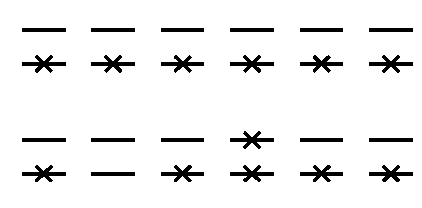
\includegraphics[width=7cm]{fig11-1.pdf}\\[0.3em]
{\small (a) 基态\qquad\qquad (b) 第一激发态}\\[0.2em]
{\small 图 11.1\quad $\Delta=0$ 时半满赫伯德模型的能态}
\end{minipage}
\end{center}

以上结果只是孤立原子系统的严格解.假如各格点上原子轨道波函数彼此重叠，则电子将在整个晶体中运动，并分别形成以 $T_{0}$ 为中心和以 $T_{0}+U$ 为中心的两个子带.当 $n=1$ 时，电子只填满 $T_{0}$ 子带，而 $T_{0}+U$ 子带则是空带，这时晶体是绝缘体.如果原子波函数重叠很厉害，则合并为一个半满能带，晶体是良导体.在中间情况，可能发生金属-绝缘体相变.

\subsection*{4. 窄带中的强关联效应}

当能带宽度 $\Delta\neq0$ 时，我们必须从严格的赫伯德哈密顿量［式(11.1.13)］出发，计入 $T_{ij}(j\neq i)$ 项.由于H不再是 $n_{i\sigma}$ 的对角型，利用格林函数方法只能求得近似解.

现在具体讨论 $\Delta\neq0$ 时的格林函数方程式(11.1.28)和式(11.1.33).从H的表示式(11.1.13)计算出下列对易式：
\begin{equation}
  [C_{i\sigma},H]=\sum_{j}T_{ij}C_{j\sigma}+Un_{i\bar{\sigma}}C_{i\sigma}
\end{equation}
\begin{equation}
\begin{aligned}
  \relax[n_{i\bar{\sigma}}C_{i\sigma},H]&=Un_{i\bar{\sigma}}C_{i\sigma}
  +T_{0}n_{i\bar{\sigma}}C_{i\sigma}
  +\sum_{l(l\neq i)}T_{il}\,n_{i\bar{\sigma}}C_{l\sigma}\\
  &\quad+\sum_{l}T_{il}
  \bigl(C^{+}_{i\bar{\sigma}}C_{l\bar{\sigma}}
  -C^{+}_{l\bar{\sigma}}C_{i\bar{\sigma}}\bigr)C_{i\sigma}
\end{aligned}
\end{equation}
将以上结果代入式(11.1.28)和(11.1.33)，所得到的运动方程并不封闭，因为式(11.1.41)中含交迭积分的项使 $\Gamma^{\sigma}_{ij}(\omega)$ 方程中出现三格点高阶格林函数.在窄带强关联情况下，为了使方程封闭，可以对这些项作如下近似处理：将式(11.1.41)右边有"~~~"号的算符部分近似用各自的平均值 $\langle n_{\bar{\sigma}}\rangle$ 和 $(\langle C^{+}_{i\bar{\sigma}}C_{l\bar{\sigma}}\rangle-\langle C^{+}_{l\bar{\sigma}}C_{i\bar{\sigma}}\rangle)$ 代替.由于 $E_{k}=E_{-k}$，可证明 $T_{il}=T_{li}$，再利用平移对称性将有
\begin{equation*}
  \sum_{l}T_{il}\bigl(\langle C^{+}_{i\bar{\sigma}}C_{l\bar{\sigma}}\rangle
  -\langle C^{+}_{l\bar{\sigma}}C_{i\bar{\sigma}}\rangle\bigr)=0
\end{equation*}
按照这样的近似方案，式(11.1.41)右边第四项的贡献为零，而第三项则给出 $G^{\sigma}_{lj}(\omega)$，这就是切断近似.由此求出近似封闭的格林函数方程组：
\begin{equation}
  \omega G^{\sigma}_{ij}(\omega)=\delta_{ij}
  +\sum_{l}T_{il}G^{\sigma}_{lj}(\omega)+U\Gamma^{\sigma}_{ij}(\omega)
\end{equation}
\begin{equation}
  \omega\Gamma^{\sigma}_{ij}(\omega)=\langle n_{\bar{\sigma}}\rangle\delta_{ij}
  +\langle n_{\bar{\sigma}}\rangle\sum_{l(l\neq i)}T_{il}G^{\sigma}_{lj}(\omega)
  +(T_{0}+U)\Gamma^{\sigma}_{ij}(\omega)
\end{equation}
由式(11.1.43)可解出
\begin{equation}
  \Gamma^{\sigma}_{ij}(\omega)=\frac{\langle n_{\bar{\sigma}}\rangle}{\omega-T_{0}-U}
  \Bigl\{\delta_{ij}+\sum_{l(l\neq i)}T_{il}G^{\sigma}_{lj}(\omega)\Bigr\}
\end{equation}
代入式(11.1.42)，得到单粒子格林函数方程
\begin{equation}
\begin{aligned}
  \omega G^{\sigma}_{ij}(\omega)&=T_{0}G^{\sigma}_{ij}(\omega)
  +\biggl\{1+\frac{U\langle n_{\bar{\sigma}}\rangle}{\omega-T_{0}-U}\biggr\}
  \bigl\{\delta_{ij}+\sum_{l(l\neq i)}T_{il}G^{\sigma}_{lj}\bigr\}\\
  &\qquad(i,\,j=1,\,2,\,\cdots,\,N)
\end{aligned}
\end{equation}
式(11.1.45)是格点格林函数 $G^{\sigma}_{ij}$ 的 $(N\times N)$ 矩阵方程，可利用表象变换求解.对于平移不变的系统，格点格林函数 $G^{\sigma}_{ij}$ 只是 $(\boldsymbol{R}_{i}-\boldsymbol{R}_{j})$ 的函数.这时利用变换式(11.1.5)可证明在布洛赫表象中单粒子格林函数是对角的，即
\begin{equation}
\begin{aligned}
  G^{\sigma}_{kk'}(\omega)&\equiv
  \langle\langle C_{k\sigma}\mid C^{+}_{k'\sigma}\rangle\rangle_{\omega}
  =N^{-1}\sum_{i,\,j}\mathrm{e}^{-\mathrm{i}\boldsymbol{k}\cdot\boldsymbol{R}_{i}}
  \mathrm{e}^{\mathrm{i}\boldsymbol{k}'\cdot\boldsymbol{R}_{j}}
  \langle\langle C_{i\sigma}\mid C^{+}_{j\sigma}\rangle\rangle_{\omega}\\
  &=\delta_{kk'}\langle\langle C_{k\sigma}\mid C^{+}_{k\sigma}\rangle\rangle_{\omega}
  \equiv\delta_{kk'}G^{\sigma}_{k}(\omega)
\end{aligned}
\end{equation}
其中 $G^{\sigma}_{k}(\omega)$ 是布洛赫表象中的对角格林函数 $\langle\langle C_{k\sigma}\mid C^{+}_{k\sigma}\rangle\rangle_{\omega}$.因此有傅里叶变换式
\begin{equation}
\begin{aligned}
  G^{\sigma}_{ij}(\omega)&=\frac{1}{N}\sum_{k}\sum_{k'}
  \mathrm{e}^{\mathrm{i}\boldsymbol{k}\cdot\boldsymbol{R}_{i}}
  \mathrm{e}^{-\mathrm{i}\boldsymbol{k}'\cdot\boldsymbol{R}_{j}}
  G^{\sigma}_{kk'}(\omega)\\
  &=\frac{1}{N}\sum_{k}\mathrm{e}^{\mathrm{i}\boldsymbol{k}\cdot(\boldsymbol{R}_{i}-\boldsymbol{R}_{j})}
  G^{\sigma}_{k}(\omega)
\end{aligned}
\end{equation}
利用上式以及式(11.1.7)的逆变换
\begin{equation}
  E_{k}=\frac{1}{N}\sum_{i,\,j}T_{ij}
  \mathrm{e}^{-\mathrm{i}\boldsymbol{k}\cdot(\boldsymbol{R}_{i}-\boldsymbol{R}_{j})}
\end{equation}
不难将式(11.1.45)对角化为格林函数 $G^{\sigma}_{k}(\omega)$ 的简单代数方程
\begin{equation}
  \omega G^{\sigma}_{k}(\omega)=T_{0}G^{\sigma}_{k}(\omega)
  +\biggl\{1+\frac{U\langle n_{\bar{\sigma}}\rangle}{\omega-T_{0}-U}\biggr\}
  \bigl\{1+(E_{k}-T_{0})G^{\sigma}_{k}(\omega)\bigr\}
\end{equation}
由此解出单粒子格林函数
\begin{equation}
  G^{\sigma}_{k}(\omega)=
  \frac{\omega-T_{0}-U(1-\langle n_{\bar{\sigma}}\rangle)}
  {(\omega-E_{k})(\omega-T_{0}-U)+\langle n_{\bar{\sigma}}\rangle U(T_{0}-E_{k})}
\end{equation}
为了讨论这个解的特点，将上式整理成下列标准形式：
\begin{equation}
  G^{\sigma}_{k}(\omega)=\frac{A^{(1)}_{k\sigma}}{\omega-E^{(1)}_{k\sigma}}
  +\frac{A^{(2)}_{k\sigma}}{\omega-E^{(2)}_{k\sigma}}
\end{equation}
其中 $E^{(1)}_{k\sigma}$ 和 $E^{(2)}_{k\sigma}$ 是格林函数 $G^{\sigma}_{k}(\omega)$ 之极点，由式(11.1.50)的分母等于零确定，即是下列二次方程的根
\begin{equation}
  (\omega-E_{k})(\omega-T_{0}-U)
  +\langle n_{\bar{\sigma}}\rangle(T_{0}-E_{k})U=0
\end{equation}
由此求出
\begin{equation}
\left.
\begin{aligned}
  &E^{(1)}_{k\sigma}\\
  &E^{(2)}_{k\sigma}
\end{aligned}\right\}
  =\frac{1}{2}\Bigl\{E_{k}+U+T_{0}
  \mp\sqrt{(E_{k}-U-T_{0})^{2}+4U\langle n_{\bar{\sigma}}\rangle(E_{k}-T_{0})}\Bigr\}
\end{equation}
并且
\begin{equation}
  E^{(1)}_{k\sigma}<T_{0}+U(1-\langle n_{\bar{\sigma}}\rangle)
  <E^{(2)}_{k\sigma}
\end{equation}
说明两支解不相交.系数 $A^{(i)}_{k\sigma}(i=1,\,2)$ 由式(11.1.50)和式(11.1.51)决定，有关系式
\begin{equation}
\begin{aligned}
  &A^{(i)}_{k\sigma}=\frac{\partial E^{(i)}_{k\sigma}}{\partial E_{k}}
  \qquad(i=1,\,2)\\
  &A^{(1)}_{k\sigma}+A^{(2)}_{k\sigma}=1
\end{aligned}
\end{equation}
具体将 $E^{(i)}_{k\sigma}$ 的表示式(11.1.53)代入上式可求得
\begin{equation}
\left.
\begin{aligned}
  &A^{(1)}_{k\sigma}\\
  &A^{(2)}_{k\sigma}
\end{aligned}\right\}
  =\frac{1}{2}\Biggl\{1\mp
  \frac{E_{k}-U-T_{0}+2U\langle n_{\bar{\sigma}}\rangle}
  {\sqrt{(E_{k}-U-T_{0})^{2}+4U\langle n_{\bar{\sigma}}\rangle(E_{k}-T_{0})}}\Biggr\}
\end{equation}
对式(11.1.39)的第一个等式作傅里叶变换，得到局域态密度的 $G^{\sigma}_{k}$ 表示式
\begin{equation}
\begin{aligned}
  \rho_{\sigma}(\omega)&=\frac{\mathrm{i}}{2\pi N}\sum_{j}
  \bigl\{G^{\sigma}_{jj}(\omega+\mathrm{i}\eta)
  -G^{\sigma}_{jj}(\omega-\mathrm{i}\eta)\bigr\}\\
  &=\frac{\mathrm{i}}{2\pi}\sum_{k}
  \bigl\{G^{\sigma}_{k}(\omega+\mathrm{i}\eta)
  -G^{\sigma}_{k}(\omega-\mathrm{i}\eta)\bigr\}
  \qquad(\eta=+0)
\end{aligned}
\end{equation}
将式(11.1.51)代入上式，可求出 $\Delta\neq0$ 时赫伯德系统中的电子态密度
\begin{equation}
  \rho_{\sigma}(\omega)=\frac{1}{N}\sum_{k}
  \bigl\{A^{(1)}_{k\sigma}\delta\bigl[\omega-E^{(1)}_{k\sigma}\bigr]
  +A^{(2)}_{k\sigma}\delta\bigl[\omega-E^{(2)}_{k\sigma}\bigr]\bigr\}
\end{equation}
仔细分析上式不难了解，由于关联作用原来的单个能带分裂为两个子能带.例如：

(i) $U=0$ 情况，即不计电子间的关联作用.直接由式(11.1.50)可得单能带解为
\begin{equation*}
  G^{\sigma}_{k}(\omega)\Big|_{U=0}=\frac{1}{\omega-E_{k}}
\end{equation*}
其极点 $E_{k}$ 就是能带电子的能量，而态密度相应为
\begin{equation}
\begin{aligned}
  \rho_{\sigma}(\omega)\Big|_{U=0}
  &=\frac{1}{N}\sum_{k}\delta(\omega-E_{k})\\
  &=\int_{-\infty}^{\infty}\mathrm{d}E_{k}\,D(E_{k})\delta(\omega-E_{k})=D(\omega)
\end{aligned}
\end{equation}
这里 $D(\omega)$ 代表单带 $E_{k}$ 的态密度.这个能带的中心在 $T_{0}$ 处，可用图11.2定性表示其能带曲线和态密度，图中 $\Delta$ 为能带宽度，并且 $\dfrac{\Delta}{2}\geqslant|E_{k}-T_{0}|$.

\begin{center}
\begin{minipage}{9cm}
\centering
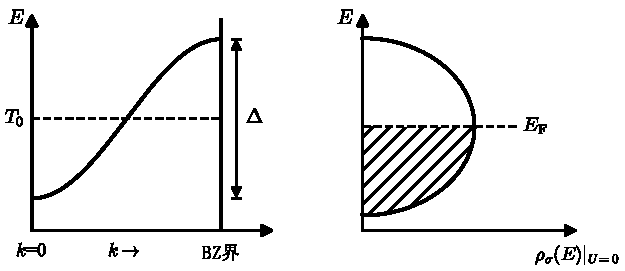
\includegraphics[width=9cm]{fig11-2.pdf}\\[0.3em]
{\small (a) 能带曲线\qquad\qquad (b) 态密度}\\[0.2em]
{\small 图 11.2\quad 不计关联时的单带示意图}
\end{minipage}
\end{center}

(ii) $U\geqslant\Delta$，即窄带中强关联情况.这时可设
\begin{equation}
  U\gg|E_{k}-T_{0}|
\end{equation}
再对式(11.1.53)和式(11.1.56)作展开，求得
\begin{equation}
\left.
\begin{aligned}
  &E^{(1)}_{k\sigma}\approx T_{0}+(E_{k}-T_{0})(1-\langle n_{\bar{\sigma}}\rangle)\\
  &E^{(2)}_{k\sigma}\approx U+T_{0}+(E_{k}-T_{0})\langle n_{\bar{\sigma}}\rangle
\end{aligned}\right\}
\end{equation}
\begin{equation}
  A^{(1)}_{k\sigma}\approx1-\langle n_{\bar{\sigma}}\rangle,
  \qquad A^{(2)}_{k\sigma}\approx\langle n_{\bar{\sigma}}\rangle
\end{equation}
格林函数和态密度的近似式为
\begin{equation}
  G^{\sigma}_{k}(\omega)\approx
  \biggl\{\frac{1-\langle n_{\bar{\sigma}}\rangle}
  {\omega-T_{0}-(E_{k}-T_{0})(1-\langle n_{\bar{\sigma}}\rangle)}
  +\frac{\langle n_{\bar{\sigma}}\rangle}
  {\omega-T_{0}-U-(E_{k}-T_{0})\langle n_{\bar{\sigma}}\rangle}\biggr\}
\end{equation}
\begin{equation}
  \rho_{\sigma}(\omega)\approx\frac{1}{N}\sum_{k}
  \bigl\{(1-\langle n_{\bar{\sigma}}\rangle)
  \delta\bigl[\omega-T_{0}-(E_{k}-T_{0})(1-\langle n_{\bar{\sigma}}\rangle)\bigr]
  +\langle n_{\bar{\sigma}}\rangle
  \delta\bigl[\omega-T_{0}-U-(E_{k}-T_{0})\langle n_{\bar{\sigma}}\rangle\bigr]\bigr\}
\end{equation}
显然，两个子带分别以 $T_{0}$ 和 $T_{0}+U$ 为中心.

对于零能带宽度情况，应取 $E_{k}=T_{0}$，这时式(11.1.64)还原为 $\Delta=0$ 情况的态密度公式(11.1.39)，而格林函数
\begin{equation}
  G^{\sigma}_{k}(\omega)\Big|_{\Delta=0}
  =\frac{1-\langle n_{\bar{\sigma}}\rangle}{\omega-T_{0}}
  +\frac{\langle n_{\bar{\sigma}}\rangle}{\omega-T_{0}-U}
\end{equation}
将上式代入表象变换式(11.1.47)，可求得格点格林函数
$G^{\sigma}_{ij}(\omega)=\delta_{ij}G^{\sigma}_{k}(\omega)\big|_{\Delta=0}$，
与孤立原子极限时的严格解［式(11.1.37)］相符.利用式(11.1.53)、(11.1.56)和(11.1.58)严格作出的能带曲线和态密度图形可参考赫伯德的原文\textsuperscript{[1]}.图11.3只是根据以上讨论所绘的示意图.

\begin{center}
\begin{minipage}{9cm}
\centering
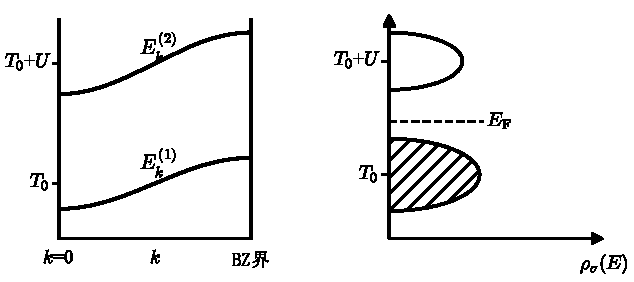
\includegraphics[width=9cm]{fig11-3.pdf}\\[0.3em]
{\small (a) 子能带曲线\qquad\qquad (b) 子带态密度的示意图}\\[0.2em]
{\small 图 11.3\quad 计入关联后的能带分裂图}
\end{minipage}
\end{center}

由以上图形可知，当 $E_{k}$ 能带为半满情况时，电子间的关联作用将使能带在费密能级 $E_{\mathrm{F}}$ 处发生分裂，从而形成两个子带，一个被填满另一个则是空带，将使金属变为绝缘体（称为M-I转变）.导致能带分裂的主要原因是同一格点周围的相反自旋电子间的库仑排斥作用，这是多体系统的强关联效应对能带的影响，可用于解释MnO及La$_{2}$CuO$_{4}$等化合物为什么是绝缘体.

\subsection*{5. 半满带中的金属-绝缘体转变}

以上讨论的一个结论是：只要计入了电子间的关联，则无论U多么小，都将导致单能带分裂为两个子带.事实上当 $U\ll\Delta$ 时这个结论是不正确的.因为从本节"3"的严格解可知，当不同格点上的原子局域轨道波函数不重叠时 $(\Delta=0)$，晶体中电子只可能处于 $T_{0}$ 和 $T_{0}+U$ 能级.当U很大而局域轨道重叠较小时 $(U\gg\Delta)$，各格点周围的 $T_{0}$ 和 $T_{0}+U$ 能级分别组成两个很窄的子能带，它们彼此不相交叠，对于 $n=1$ 情况（电子数$=$格点数），晶体仍为绝缘体.假如U较小而轨道波函数的重叠又很厉害，以至 $\Delta\gg U$，则以 $T_{0}$ 为中心和以 $T_{0}+U$ 为中心的两个子能带将彼此相交和重叠，实际上成为一个半填满的能带，这时晶体表现出金属性.因此，在半满能带 $E_{k}$ 中当计入电子关联作用后倒底是金属性的晶体(M)，还是绝缘体(I)取决于U和 $\Delta$ 的相对大小，在某个确定的比值 $(\Delta/U)_{\mathrm{c}}$ 处将发生M-I转变.

本节"4"中的理论之所以不能给出M-I转变的条件，是由于建立 $\Gamma^{\sigma}_{ij}(\omega)$ 的方程(11.1.43)时所采用的近似过于粗糙，忽略了子带的变宽效应.假如比(4)中处理更进一步，不对 $\Gamma^{\sigma}_{ij}(\omega)$ 方程作近似，而是写出严格的 $\Gamma^{\sigma}_{ij}(\omega)$ 方程.然后，再写出第三套格林函数锁链方程并对第三套方程作切断近似，使方程组封闭，则可以求得M-I转变的条件，这就是赫伯德后一个工作\textsuperscript{[3]}的要点.文献[3]中所求出的能带参量与 $(\Delta/U)$ 的关系如图11.4，当 $(\Delta/U)<\dfrac{2}{\sqrt{3}}$ 时半满带分裂为两个子带，系统表现出绝缘体特性.在相反的情况 $(\Delta/U)>\dfrac{2}{\sqrt{3}}$ 时，能带不分裂，晶体具有金属性.因此，$(\Delta/U)_{\mathrm{c}}=\dfrac{2}{\sqrt{3}}$ 是M-I转变点.这样用赫伯德模型就能够解释；同样是具有未填满d带的过渡金属氧化物，为什么有些是良导体，而另一些则是绝缘体.

\begin{center}
\begin{minipage}{6.5cm}
\centering
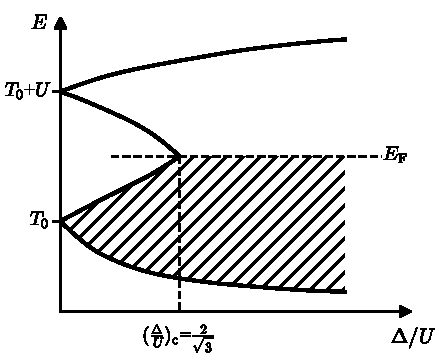
\includegraphics[width=6.5cm]{fig11-4.pdf}\\{\small 图 11.4\quad 赫伯德模型中的 M-I转变}
\end{minipage}
\end{center}

近年来赫伯德模型广泛用于强关联电子体系，发展了著名的t-J模型（见本章§9），用于建立铜氧化合物的高温超导理论（见本章§10）.此外，赫伯德模型还适用于讨论金属磁性问题，并在20世纪80年代初期发展了巡游电子磁性的自旋涨落理论，我们将在§11中作简要介绍.

\section{局域磁矩理论}

最简单的杂质局域态是半导体中的施主或受主能级状态，在第八章中我们曾经用有效哈密顿量讨论了这个问题.在那里杂质只是当作一个受到介质屏蔽的有心力势场处理，忽略了基质晶体中电子与杂质原子上电子之间的相互转移和状态混合效应.当基质晶体为金属、杂质是过渡族磁性原子时，状态的混合作用特别重要，它涉及金属中局域磁矩的形成问题，是局域态理论的一个重要方面.

大家知道，具有未填满d壳层的过渡元素，由于电子间的库仑排斥作用，d电子自旋矩按照洪德（Hund）定则排列，从而形成自由原子的固有磁矩.试问磁性原子溶入非磁性金属基体后是否仍保持原子的磁性状态？表11.1是局域磁矩的测量结果，表中还列出了基体金属的费密能 $E_{\mathrm{F}}$.

表 11.1\quad 金属基体中的杂质磁矩

{\small （"+"——有局域磁性，"$-$"——无局域磁矩，"？"——不明）}

\begin{center}\small
\begin{tabular}{lcccc}
\hline
磁性原子＼基体金属 & Au & Cu & Zn & Al\\
\hline
Mn & $+$ & $+$ & $+$ & $-$\\
Cr & $+$ & $+$ & $+$ & $-$\\
Fe & $+$ & $+$ & $-$ & $-$\\
Co & $?$ & $?$ & $?$ & $-$\\
Ni & $-$ & $-$ & $-$ & $-$\\
$E_{\mathrm{F}}$/eV & 5.5 & 7 & 9.5 & 13\\
\hline
\end{tabular}
\end{center}

显然，情况相当复杂，磁性原子溶入金属后并不都形成局域磁矩.例如，Fe溶于Cu中有局域磁矩，但Ni溶于Cu中就不产生局域磁性.又如，同样的磁性原子Mn在金属Cu中可测得局域磁矩，而在金属Al中室温下几乎测不出Mn的磁矩.因此，需要一个理论来说明在什么条件下金属中可形成局域磁矩？

\subsection*{1. 安德逊哈密顿量}

1961年安德逊\textsuperscript{[4]}提出了s-d混合模型（s-d mixing model），他认为在非磁性的金属基体中讨论过渡族杂质原子形成局域磁矩必须同时考虑两方面的因素：其一，和自由原子形成固有磁矩相似，杂质原子中d壳层电子的库仑作用对晶体形成局域磁矩有重要影响；其二，由于在晶体中杂质的自由原子d轨道状态 $\phi_{\mathrm{L}}(\boldsymbol{r})$ 不再是严格的本征态，特别是由于在金属晶体中存在着电子退局域化（delocalized）为布洛赫轨道态（s轨道）的倾向，$\phi_{\mathrm{L}}$ 与 $\phi_{k}$ 态之间存在着电子的相互转移，安德逊称之为s-d混合作用.为此，他指出系统的哈密顿量H应由下列四部分组成：

(i) 金属中能带电子的哈密顿量为
\begin{equation}
  \sum_{k,\,\sigma}E_{k}n_{k\sigma}
  \qquad(n_{k\sigma}=C^{+}_{k\sigma}C_{k\sigma})
\end{equation}
$E_{k}$ 代表布洛赫轨道电子能量，$C_{k\sigma}$ 是布洛赫表象中电子的消灭算符.

(ii) 杂质原子的未微扰d态哈密顿量为
\begin{equation}
  \sum_{\sigma}E_{\mathrm{d}}n_{\mathrm{d}}
  \qquad(n_{\mathrm{d}}=d^{+}_{\sigma}d_{\sigma})
\end{equation}
$d^{+}_{\sigma}$ 和 $d_{\sigma}$ 代表 $\phi_{\mathrm{L}}$ 轨道上 $\sigma$ 自旋的d电子的产生和消灭算符，$E_{\mathrm{d}}$ 是d态为单占据时的能量.即使是讨论孤立原子的磁矩形成问题，我们也必须考虑电子间的库仑关联作用，为简单起见设d态是非简并的，在反向自旋的d态电子之间有库仑排斥作用.因此

(iii) 关联作用项可写成
\begin{equation}
\begin{aligned}
  &Un_{\mathrm{d}\uparrow}n_{\mathrm{d}\downarrow}
  =\frac{U}{2}\sum_{\sigma}n_{\mathrm{d}\sigma}n_{\mathrm{d}\bar{\sigma}}\\
  &U=\int|\phi_{\mathrm{L}}(\boldsymbol{r})|^{2}
  |\phi_{\mathrm{L}}(\boldsymbol{r}')|^{2}
  \frac{e^{2}}{|\boldsymbol{r}-\boldsymbol{r}'|}
  \,\mathrm{d}\boldsymbol{r}\,\mathrm{d}\boldsymbol{r}'
\end{aligned}
\end{equation}
这里U是d电子的关联能.根据上节的讨论，如果 $E_{\mathrm{d}}$ 为第一个d电子的能量，则第二个自旋取向相反的电子在d态上的能量必为 $E_{\mathrm{d}}+U$，能量差U是形成磁矩的一个重要原因.但是，在金属中还存在 $\phi_{\mathrm{L}}$ 与 $\phi_{k}$ 态间的电子转移效应，其作用可表示为

(iv) s-d混合项
\begin{equation}
  \sum_{k,\,\sigma}V_{kd}
  \bigl(C^{+}_{k\sigma}d_{\sigma}+d^{+}_{\sigma}C_{k\sigma}\bigr)
\end{equation}
它代表布洛赫态与局域态之间的转移，是纯粹的单电子效应.$V_{kd}$ 称为s-d混合强度，来源于 $\phi_{\mathrm{L}}$ 与 $\phi_{k}$ 彼此不正交，可表示为
\begin{equation*}
\begin{aligned}
  V_{kd}&=\langle\phi_{\mathrm{L}}(\boldsymbol{r})|\mathscr{H}|\phi_{k}(\boldsymbol{r})\rangle\\
  &=\frac{1}{\sqrt{N}}\sum_{l}\mathrm{e}^{\mathrm{i}\boldsymbol{k}\cdot\boldsymbol{R}_{l}}
  \langle\phi_{\mathrm{L}}(\boldsymbol{r})|\mathscr{H}
  |a(\boldsymbol{r}-\boldsymbol{R}_{l})\rangle
\end{aligned}
\end{equation*}
其中杂质位于原点，$\mathscr{H}$ 是单电子哈密顿量，$a(\boldsymbol{r}-\boldsymbol{R}_{l})$ 是金属中能带电子的瓦尼尔函数.从第二个等式还可以看出，s-d混合作用与紧束缚近似中不同格点间电子的转移作用非常相似，其中 $\boldsymbol{R}_{l}=0$ 项对 $V_{kd}$ 无贡献，这是因为局域的d态函数 $\phi_{\mathrm{L}}(\boldsymbol{r})$ 与属于导带并以原点为中心的瓦尼尔函数 $a(\boldsymbol{r})$ 彼此是正交的.

综合以上四部分，再计入外加均匀磁场h的作用，得到总哈密顿量
\begin{equation}
\begin{aligned}
  H&=\sum_{k,\,\sigma}E_{k\sigma}n_{k\sigma}
  +\sum_{\sigma}E_{\mathrm{d}\sigma}n_{\mathrm{d}\sigma}
  +\frac{U}{2}\sum_{\sigma}n_{\mathrm{d}\sigma}n_{\mathrm{d}\bar{\sigma}}\\
  &\quad+\sum_{k,\,\sigma}V_{kd}
  \bigl(C^{+}_{k\sigma}d_{\sigma}+d^{+}_{\sigma}C_{k\sigma}\bigr)
\end{aligned}
\end{equation}
其中
\begin{equation}
  E_{k\sigma}=E_{k}+\sigma\mu_{\mathrm{B}}h,
  \qquad E_{\mathrm{d}\sigma}=E_{\mathrm{d}}+\sigma\mu_{\mathrm{B}}h
\end{equation}
这里 $\mu_{\mathrm{B}}=\dfrac{|e|\hbar}{2mc}$ 为玻尔磁子，并设电子与杂质的朗德（Landé）因子 $g_{0}=g_{i}=2$，这就是轨道非简并的安德逊s-d混合模型.

\subsection*{2. 安德逊s-d混合模型的格林函数}

从双时推迟格林函数
\begin{equation*}
  \langle\langle A(t);B(t')\rangle\rangle
  =-\mathrm{i}\theta(t-t')
  \langle[A(t),B(t')]_{+}\rangle
\end{equation*}
出发，利用一个技巧，对函数 $\langle\langle A(t);B(t')\rangle\rangle$ 分别求t及 $t'$ 的微商，可求得下列两个运动方程：
\begin{equation}
  \mathrm{i}\frac{\mathrm{d}}{\mathrm{d}t}
  \langle\langle A(t);B(t')\rangle\rangle
  =\delta(t-t')\langle[A,B]_{+}\rangle
  +\langle\langle[A,H];B(t')\rangle\rangle
\end{equation}
\begin{equation}
  -\mathrm{i}\frac{\mathrm{d}}{\mathrm{d}t'}
  \langle\langle A(t);B(t')\rangle\rangle
  =\delta(t-t')\langle[A,B]_{+}\rangle
  +\langle\langle A(t);[B,H]\rangle\rangle
\end{equation}
作傅里叶变换
\begin{equation}
  \langle\langle A\mid B\rangle\rangle_{\omega}
  =\int\mathrm{d}t\,\mathrm{e}^{\mathrm{i}\omega(t-t')}
  \langle\langle A(t);B(t')\rangle\rangle
\end{equation}
可得到格林函数运动方程通式的两种表示式
\begin{equation}
  \omega\langle\langle A\mid B\rangle\rangle_{\omega}
  =\langle[A,B]_{+}\rangle
  +\langle\langle[A,H]\mid B\rangle\rangle_{\omega}
\end{equation}
\begin{equation}
  \omega\langle\langle A\mid B\rangle\rangle_{\omega}
  =\langle[A,B]_{+}\rangle
  -\langle\langle A\mid[B,H]\rangle\rangle_{\omega}
\end{equation}
用它们处理s-d混合模型比较方便\textsuperscript{[5]}.

我们的目的是要找出形成局域磁矩的条件，即讨论系统在什么条件下有 $\langle n_{\mathrm{d}\uparrow}\rangle\neq\langle n_{\mathrm{d}\downarrow}\rangle$ 解？为此，应建立单粒子格林函数 $\langle\langle d_{\sigma}\mid d^{+}_{\sigma}\rangle\rangle_{\omega}$ 和 $\langle\langle C_{k\sigma}\mid C^{+}_{k\sigma}\rangle\rangle_{\omega}$ 的运动方程，利用式(11.2.10)写出
\begin{equation}
  (\omega-E_{k\sigma})
  \langle\langle C_{k\sigma}\mid C^{+}_{k'\sigma}\rangle\rangle_{\omega}
  =\delta_{k,\,k'}
  +V_{kd}\langle\langle d_{\sigma}\mid C^{+}_{k'\sigma}\rangle\rangle_{\omega}
\end{equation}
\begin{equation}
\begin{aligned}
  (\omega-E_{\mathrm{d}\sigma})
  \langle\langle d_{\sigma}\mid d^{+}_{\sigma}\rangle\rangle_{\omega}
  &=1+U\langle\langle n_{\mathrm{d}\bar{\sigma}}d_{\sigma}
  \mid d^{+}_{\sigma}\rangle\rangle_{\omega}\\
  &\quad+\sum_{k}V_{kd}
  \langle\langle C_{k\sigma}\mid d^{+}_{\sigma}\rangle\rangle_{\omega}
\end{aligned}
\end{equation}
对于混合格林函数 $\langle\langle C_{k\sigma}\mid d^{+}_{\sigma}\rangle\rangle_{\omega}$，仍通过式(11.2.10)写运动方程
\begin{equation}
  (\omega-E_{k\sigma})
  \langle\langle C_{k\sigma}\mid d^{+}_{\sigma}\rangle\rangle_{\omega}
  =V_{kd}\langle\langle d_{\sigma}\mid d^{+}_{\sigma}\rangle\rangle_{\omega}
\end{equation}
另一个混合格林函数 $\langle\langle d_{\sigma}\mid C^{+}_{k\sigma}\rangle\rangle_{\omega}$ 则利用第二套运动方程的通式(11.2.11)，求得
\begin{equation}
  (\omega-E_{k'\sigma})
  \langle\langle d_{\sigma}\mid C^{+}_{k'\sigma}\rangle\rangle_{\omega}
  =V_{k'd}\langle\langle d_{\sigma}\mid d^{+}_{\sigma}\rangle\rangle_{\omega}
\end{equation}
如果对方程(11.2.13)中的高阶格林函数作切断近似：
\begin{equation}
  \langle\langle n_{\mathrm{d}\bar{\sigma}}d_{\sigma}\mid d^{+}_{\sigma}\rangle\rangle_{\omega}
  \approx\langle n_{\mathrm{d}\bar{\sigma}}\rangle
  \langle\langle d_{\sigma}\mid d^{+}_{\sigma}\rangle\rangle_{\omega}
\end{equation}
将得到近似式
\begin{equation}
  (\omega-E_{\mathrm{d}\sigma}-U\langle n_{\mathrm{d}\bar{\sigma}}\rangle)
  \langle\langle d_{\sigma}\mid d^{+}_{\sigma}\rangle\rangle_{\omega}
  =1+\sum_{k}V_{kd}
  \langle\langle C_{k\sigma}\mid d^{+}_{\sigma}\rangle\rangle_{\omega}
\end{equation}
这时式(11.2.12)、式(11.2.14)、式(11.2.15)和(11.2.17)构成近似封闭的格林函数方程组，格林函数可解出.切断近似式(11.2.16)相当于对H中的关联项作下列线性化近似：
\begin{equation}
  \frac{U}{2}\sum_{\sigma}n_{\mathrm{d}\sigma}n_{\mathrm{d}\bar{\sigma}}
  \approx U\sum_{\sigma}\langle n_{\mathrm{d}\bar{\sigma}}\rangle n_{\mathrm{d}\sigma}
  -U\langle n_{\mathrm{d}\uparrow}\rangle\langle n_{\mathrm{d}\downarrow}\rangle
\end{equation}
显然这就是哈特利-福克近似.因此，用上述切断近似所建立的格林函数封闭方程组属于哈特利-福克近似(HFA).

现在求格林函数的HFA解.将式(11.2.15)代入式(11.2.12)，求得
\begin{equation}
  \langle\langle C_{k\sigma}\mid C^{+}_{k'\sigma}\rangle\rangle_{\omega}
  =\frac{\delta_{kk'}}{(\omega-E_{k\sigma})}
  +\frac{V_{kd}V_{k'd}}{(\omega-E_{k\sigma})(\omega-E_{k'\sigma})}
  \langle\langle d_{\sigma}\mid d^{+}_{\sigma}\rangle\rangle_{\omega}
\end{equation}
其中等式右边第一项为自由粒子的格林函数，第二项代表s-d混合作用的影响.格林函数 $\langle\langle d_{\sigma}\mid d^{+}_{\sigma}\rangle\rangle_{\omega}$ 由式(11.2.14)代入近似式(11.2.17)，消去 $\langle\langle C_{k\sigma}\mid d^{+}_{\sigma}\rangle\rangle_{\omega}$ 后为
\begin{equation}
  \langle\langle d_{\sigma}\mid d^{+}_{\sigma}\rangle\rangle_{\omega}
  =\frac{1}{\omega-E_{\mathrm{d}\sigma}
  -U\langle n_{\mathrm{d}\bar{\sigma}}\rangle-F_{\sigma}(\omega)}
\end{equation}
对于推迟格林函数应取 $\omega+\mathrm{i}\eta$.在上式中
\begin{equation}
\begin{aligned}
  F_{\sigma}(\omega+\mathrm{i}\eta)
  &=\sum_{k}\frac{V^{2}_{k\sigma}}{(\omega-E_{k\sigma}+\mathrm{i}\eta)}
  \qquad(\eta=+0)\\
  &=\mathscr{P}\int\frac{\rho^{(0)}(E)}{\omega-E}V^{2}_{kd}\,\mathrm{d}E
  -\mathrm{i}\pi V^{2}_{kd}\rho^{(0)}(\omega)\\
  &\approx-\mathrm{i}\pi V^{2}_{kd}\rho^{(0)}(\omega)
\end{aligned}
\end{equation}
$\rho^{(0)}(E)$ 是能带电子的态密度，可近似取其费密面上值 $\rho^{(0)}_{\mathrm{F}}$，而主值积分 $\mathscr{P}\int(\cdots)\,\mathrm{d}E$ 项的贡献很小，可以略去（或归并到 $E_{\mathrm{d}\sigma}$ 中）.定义常数
\begin{equation}
  \Gamma\equiv\pi V^{2}_{kd}\rho^{(0)}_{\mathrm{F}}
\end{equation}
将d电子格林函数的哈特利-福克近似解写成
\begin{equation}
  \langle\langle d_{\sigma}\mid d^{+}_{\sigma}\rangle\rangle_{\omega+\mathrm{i}\eta}
  =\frac{1}{\omega-E_{\mathrm{d}\sigma}
  -U\langle n_{\mathrm{d}\bar{\sigma}}\rangle+\mathrm{i}\Gamma}
\end{equation}
\begin{equation}
  \langle\langle d_{\sigma}\mid d^{+}_{\sigma}\rangle\rangle_{\omega-\mathrm{i}\eta}
  =\frac{1}{\omega-E_{\mathrm{d}\sigma}
  -U\langle n_{\mathrm{d}\bar{\sigma}}\rangle-\mathrm{i}\Gamma}
\end{equation}
再把它们代入式(11.2.19)，即可求出布洛赫电子的格林函数近似解.式(11.2.23)表明，d电子推迟格林函数的极点在复平面上 $(E_{\mathrm{d}\sigma}+U\langle n_{\mathrm{d}\bar{\sigma}}\rangle)-\mathrm{i}\Gamma$ 处，$\Gamma$ 与s-d混合作用强度有关.在这里库仑作用改变极点之实部，使能级移动，而s-d混合则使极点离开实轴，导致d电子的有限寿命 $\Gamma^{-1}$.因为对d电子的推迟格林函数式(11.2.23)作傅里叶变换，类似于附录D中式(D.22)，可写出含时的d电子推迟格林函数
\begin{equation*}
\begin{aligned}
  G_{\mathrm{r}}(t)&=\frac{1}{2\pi}\int_{-\infty}^{\infty}\mathrm{d}\omega\,
  \frac{\mathrm{e}^{-\mathrm{i}\omega t}}{\omega-\tilde{E}_{\mathrm{d}\sigma}+\mathrm{i}\Gamma}\\
  &=-\mathrm{i}\theta(t)\mathrm{e}^{-\mathrm{i}\tilde{E}_{\mathrm{d}\sigma}t}
  \mathrm{e}^{-\Gamma t}
\end{aligned}
\end{equation*}
其中
\begin{equation*}
  \tilde{E}_{\mathrm{d}\sigma}\equiv E_{\mathrm{d}\sigma}
  +U\langle n_{\mathrm{d}\bar{\sigma}}\rangle
\end{equation*}
显然，d电子在传播过程中将衰减，其寿命正比于 $\Gamma^{-1}$.

\subsection*{3. 静态磁化率}

系统的静态磁化率应包括布洛赫能带态电子和局域态d电子的贡献.因此
\begin{equation}
  \chi=\lim_{h\to0}\biggl\{\sum_{k}
  \bigl(\langle C^{+}_{k\downarrow}C_{k\downarrow}\rangle
  -\langle C^{+}_{k\uparrow}C_{k\uparrow}\rangle\bigr)\frac{\mu_{\mathrm{B}}}{h}
  +\bigl(\langle d^{+}_{\downarrow}d_{\downarrow}\rangle
  -\langle d^{+}_{\uparrow}d_{\uparrow}\rangle\bigr)\frac{\mu_{\mathrm{B}}}{h}\biggr\}
\end{equation}
其中平均量 $\langle BA\rangle$ 由谱定理决定，记为 $\mathscr{F}_{\omega}(\langle\langle A\mid B\rangle\rangle_{\omega})$
\begin{equation}
\begin{aligned}
  \langle\,BA\,\rangle&=\frac{\mathrm{i}}{2\pi}\int_{-\infty}^{\infty}
  \bigl\{\langle\langle A\mid B\rangle\rangle_{\omega+\mathrm{i}\eta}
  -\langle\langle A\mid B\rangle\rangle_{\omega-\mathrm{i}\eta}\bigr\}
  f(\omega)\,\mathrm{d}\omega\\
  &\equiv\mathscr{F}_{\omega}(\langle\langle A\mid B\rangle\rangle_{\omega})
\end{aligned}
\end{equation}
根据式(11.2.19)，磁化率可写成
\begin{equation}
  \chi=\chi_{\mathrm{p}}+\lim_{h\to0}\sum_{\sigma=\pm1}\frac{\sigma\mu_{\mathrm{B}}}{h}
  \biggl\{\sum_{k}\mathscr{F}_{\omega}\biggl[\frac{V^{2}_{kd}}{(\omega-E_{k\sigma})^{2}}
  \langle\langle d_{\sigma}\mid d^{+}_{\sigma}\rangle\rangle_{\omega}\biggr]
  +\mathscr{F}_{\omega}\bigl[\langle\langle d_{\sigma}\mid d^{+}_{\sigma}\rangle\rangle_{\omega}\bigr]\biggr\}
\end{equation}
上式中 $\chi_{\mathrm{p}}$ 项代表式(11.2.19)中自由粒子格林函数的贡献，读者不难证明它就是自由电子的泡利磁化率.式(11.2.27)中第一个 $\mathscr{F}_{\omega}$ 项的贡献可证明为零.这是因为对 $\omega$ 积分与对k求和可对调，于是在 $\omega$ 积分中有下列被积函数因子：
\begin{equation*}
  \sum_{k}\frac{V^{2}_{kd}}{(\omega-E_{k\sigma}\pm\mathrm{i}\eta)^{2}}
  =\int_{-\infty}^{\infty}
  \frac{\rho^{(0)}(E)|V_{kd}|^{2}}{(\omega-E\pm\mathrm{i}\eta)^{2}}\,\mathrm{d}E
\end{equation*}
若将 $\rho^{(0)}(E)$ 和 $|V_{kd}|^{2}$ 近似当作与E无关的常数，则这个积分的贡献为零.因此式(11.2.27)中第二项可略去.这样，除泡利磁化率外，只需再计算d电子对磁化率的贡献.将d电子的格林函数解式(11.2.23)和式(11.2.24)代入谱定理公式(11.2.26)，得
\begin{equation}
\begin{aligned}
  \mathscr{F}_{\omega}\bigl[\langle\langle d_{\sigma}\mid d^{+}_{\sigma}\rangle\rangle_{\omega}\bigr]
  &=\langle d^{+}_{\sigma}d_{\sigma}\rangle
  =\langle n_{\mathrm{d}\sigma}\rangle\\
  &=\frac{1}{\pi}\int_{-\infty}^{\infty}\mathrm{d}\omega\,f(\omega)
  \biggl\{\frac{\Gamma}{(\omega-\tilde{E}_{\mathrm{d}\sigma})^{2}+\Gamma^{2}}\biggr\}\\
  &\equiv\int_{-\infty}^{\infty}\mathrm{d}\omega\,f(\omega)\rho_{\mathrm{d}\sigma}(\omega)
\end{aligned}
\end{equation}
其中 $\rho_{\mathrm{d}\sigma}(\omega)$ 代表 $\sigma$ 自旋的d电子的态密度
\begin{equation}
  \rho_{\mathrm{d}\sigma}(\omega)=\frac{1}{\pi}
  \frac{\Gamma}{(\omega-\tilde{E}_{\mathrm{d}\sigma})^{2}+\Gamma^{2}}
\end{equation}
这里
\begin{equation}
  \tilde{E}_{\mathrm{d}\sigma}=E_{\mathrm{d}}+\sigma\mu_{\mathrm{B}}h
  +U\langle n_{\mathrm{d}\bar{\sigma}}\rangle
\end{equation}
由图11.5可知，$\rho_{\mathrm{d}\sigma}$ 是半宽度为 $\Gamma$ 的共振峰，峰的中心在 $\tilde{E}_{\mathrm{d}\sigma}$ 处，称为洛仑兹型（Lorentzian）态密度.这时金属中d电子不再是具有确定能级并且态密度为 $\delta$ 函数的束缚态，而是能级分布在 $\tilde{E}_{\mathrm{d}\sigma}$ 周围 $2\Gamma$ 宽度内的共振态（resonance state），由于它仍具有局域特性，有时也称之为虚束缚态（virtual bound state）.

\begin{center}
\begin{minipage}{4.5cm}
\centering
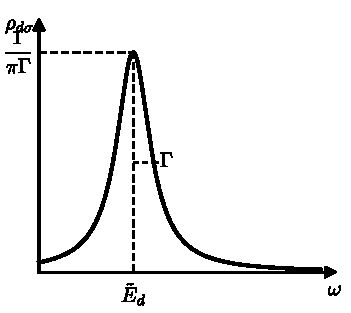
\includegraphics[width=4.5cm]{fig11-5.pdf}\\{\small 图 11.5\quad 局域电子态密度}
\end{minipage}
\end{center}

利用态密度可以计算 $T=0$ K时d态上的平均占据数.由于零温费密分布为
\begin{equation}
  f(\omega)=\begin{cases}1&(E<E_{\mathrm{F}})\\0&(E>E_{\mathrm{F}})\end{cases}
\end{equation}
代入式(11.2.28)，求得
\begin{equation}
  \langle n_{\mathrm{d}\sigma}\rangle
  =\int_{-\infty}^{E_{\mathrm{F}}}\rho_{\mathrm{d}\sigma}(\omega)\,\mathrm{d}\omega
  =\frac{1}{\pi}\mathrm{arccot}
  \biggl(\frac{\tilde{E}_{\mathrm{d}\sigma}-E_{\mathrm{F}}}{\Gamma}\biggr)
\end{equation}
式(11.2.32)实际上是自洽方程组
\begin{equation}
\left.
\begin{aligned}
  \langle n_{\mathrm{d}\uparrow}\rangle
  &=\frac{1}{\pi}\mathrm{arccot}
  \biggl[\frac{E_{\mathrm{d}}-E_{\mathrm{F}}
  +U\langle n_{\mathrm{d}\downarrow}\rangle+\mu_{\mathrm{B}}h}{\Gamma}\biggr]\\
  \langle n_{\mathrm{d}\downarrow}\rangle
  &=\frac{1}{\pi}\mathrm{arccot}
  \biggl[\frac{E_{\mathrm{d}}-E_{\mathrm{F}}
  +U\langle n_{\mathrm{d}\uparrow}\rangle-\mu_{\mathrm{B}}h}{\Gamma}\biggr]
\end{aligned}\right\}
\end{equation}
当 $h=0$ 时，如果求得 $\langle n_{\mathrm{d}\uparrow}\rangle\neq\langle n_{\mathrm{d}\downarrow}\rangle$ 解，就说明有局域磁矩，而 $\langle n_{\mathrm{d}\uparrow}\rangle=\langle n_{\mathrm{d}\downarrow}\rangle$ 解则代表无局域磁矩情况.但是，从式(11.2.33)往往同时求得有磁矩与无磁矩两种解.这时还需要一个判据确定那种解是稳定的.最简单的办法是从系统的顺磁磁化率来作判断.为此讨论杂质的非磁情况，考虑外磁场 $h=0$ 时，式(11.2.33)有非磁解
\begin{equation}
  \langle n_{\mathrm{d}\uparrow}\rangle
  =\langle n_{\mathrm{d}\downarrow}\rangle=n_{0}
\end{equation}
则在弱磁场作用时可设
\begin{equation}
\left.
\begin{aligned}
  &\langle n_{\mathrm{d}\uparrow}\rangle=n_{0}-h\Delta\\
  &\langle n_{\mathrm{d}\downarrow}\rangle=n_{0}+h\Delta
\end{aligned}\right\}
\end{equation}
外场产生的磁化正比于
\begin{equation}
  \langle n_{\mathrm{d}\downarrow}\rangle
  -\langle n_{\mathrm{d}\uparrow}\rangle=2h\Delta
\end{equation}
将式(11.2.33)对h作展开，并利用式(11.2.29)和式(11.2.36)定出未知量
\begin{equation}
  \Delta=\mu_{\mathrm{B}}
  \frac{\rho_{\mathrm{d}\sigma}(E_{\mathrm{F}})}
  {1-U\rho_{\mathrm{d}\sigma}(E_{\mathrm{F}})}
\end{equation}
根据式(11.2.27)，系统的顺磁磁化率为
\begin{equation*}
  \chi=\chi_{\mathrm{P}}+\chi_{\mathrm{I}}
\end{equation*}
$\chi_{\mathrm{I}}$ 代表杂质上d电子的磁化率，大小为
\begin{equation}
\begin{aligned}
  \chi_{\mathrm{I}}
  &=\lim_{h\to0}\bigl(\langle n_{\mathrm{d}\downarrow}\rangle
  -\langle n_{\mathrm{d}\uparrow}\rangle\bigr)\frac{\mu_{\mathrm{B}}}{h}\\
  &=2\mu^{2}_{\mathrm{B}}
  \frac{\rho_{\mathrm{d}\sigma}(E_{\mathrm{F}})}
  {1-U\rho_{\mathrm{d}\sigma}(E_{\mathrm{F}})}
\end{aligned}
\end{equation}
其中 $\rho_{\mathrm{d}\sigma}(E_{\mathrm{F}})$ 是 $\langle n_{\mathrm{d}\uparrow}\rangle=\langle n_{\mathrm{d}\downarrow}\rangle=n_{0}$ 情况下的d电子态密度，写为
\begin{equation}
\begin{aligned}
  \rho_{\mathrm{d}\sigma}(E_{\mathrm{F}})
  &=\frac{1}{\pi}
  \frac{\Gamma}{(E_{\mathrm{d}}+Un_{0}-E_{\mathrm{F}})^{2}+\Gamma^{2}}\\
  &=\frac{1}{\pi}\frac{1}{\Gamma[1+\cot^{2}(\pi n_{0})]}
  =\frac{1}{\pi}\frac{\sin^{2}\pi n_{0}}{\Gamma}
\end{aligned}
\end{equation}
在这里利用了公式
\begin{equation}
  n_{0}=\frac{1}{\pi}\mathrm{arccot}
  \biggl[\frac{E_{\mathrm{d}}+Un_{0}-E_{\mathrm{F}}}{\Gamma}\biggr]
\end{equation}
它代表无外场时式(11.2.33)有 $\langle n_{\mathrm{d}\uparrow}\rangle=\langle n_{\mathrm{d}\downarrow}\rangle$ 非磁解的情况.

由于 $T=0$ K时泡利磁化率为常数，并且它与U和 $\Gamma$ 无关.杂质磁化率 $\chi_{\mathrm{I}}$ 根据式(11.2.38)和(11.2.39)可写成
\begin{equation}
  \chi_{\mathrm{I}}=2\mu^{2}_{\mathrm{B}}
  \frac{\rho_{\mathrm{d}\sigma}(E_{\mathrm{F}})}
  {1-U\rho_{\mathrm{d}\sigma}(E_{\mathrm{F}})}
  =2\mu^{2}_{\mathrm{B}}
  \frac{1}{\biggl[\dfrac{\pi\Gamma}{\sin^{2}n_{0}\pi}-U\biggr]}
\end{equation}
上式仅仅在 $U\rho_{\mathrm{d}\sigma}(E_{\mathrm{F}})<1$ 时成立，这时 $\chi_{\mathrm{I}}>0$，对应于自由能极小，因此非磁解是稳定的，反过来当 $U\rho_{\mathrm{d}\sigma}(E_{\mathrm{F}})>1$ 时，非磁解
$\langle n_{\mathrm{d}\uparrow}\rangle_{h=0}
=\langle n_{\mathrm{d}\downarrow}\rangle_{h=0}$
不再是稳定的.由此推论，当 $U\rho_{\mathrm{d}\sigma}(E_{\mathrm{F}})>1$ 时，只可能有
$\langle n_{\mathrm{d}\uparrow}\rangle_{h=0}
\neq\langle n_{\mathrm{d}\downarrow}\rangle_{h=0}$
的磁性解.磁化率 $\chi_{\mathrm{I}}$ 的发散点出现在
\begin{equation}
  U\rho_{\mathrm{d}\sigma}(E_{\mathrm{F}})=1
  \quad\text{或}\quad
  U=\frac{\pi\Gamma}{\sin^{2}\pi n_{0}}
\end{equation}
处，它代表金属中杂质的非磁性与磁性状态的转变边界.

\subsection*{4. 局域磁矩的存在}

为了证实以上推论，我们现在讨论 $h=0$ 时自洽方程式(11.2.33)的磁性及非磁解.将式(11.2.33)的两个方程改写为下列形式：
\begin{equation}
  \langle n_{\mathrm{d}\uparrow}\rangle
  =\frac{\Gamma}{U}\cot\bigl[\pi\langle n_{\mathrm{d}\downarrow}\rangle\bigr]
  +\frac{E_{\mathrm{F}}-E_{\mathrm{d}}}{U}
\end{equation}
\begin{equation}
  \langle n_{\mathrm{d}\downarrow}\rangle
  =\frac{\Gamma}{U}\cot\bigl[\pi\langle n_{\mathrm{d}\uparrow}\rangle\bigr]
  +\frac{E_{\mathrm{F}}-E_{\mathrm{d}}}{U}
\end{equation}
并利用作图法求解.具体步骤：对给定的参数值 $\Gamma/U$ 和 $(E_{\mathrm{F}}-E_{\mathrm{d}})/U$，分别由式(11.2.43)和式(11.2.44)作 $\langle n_{\mathrm{d}\uparrow}\rangle$ 随 $\langle n_{\mathrm{d}\downarrow}\rangle$ 的变化曲线，两曲线的交点代表自洽方程的解.图11.6(a)和(b)为参数取下列值的解：
\begin{equation}
  E_{\mathrm{F}}-E_{\mathrm{d}}=\frac{U}{2}
  \quad\text{和}\quad
  \frac{\Gamma}{U}=
  \begin{cases}1&\text{(a)}\\[0.3em] \dfrac{1}{5}&\text{(b)}\end{cases}
\end{equation}
显然，在情况(a)只有非磁解
\begin{equation*}
  \langle n_{\mathrm{d}\uparrow}\rangle
  =\langle n_{\mathrm{d}\downarrow}\rangle
  =\frac{1}{2}=n_{0}
\end{equation*}
这时根据式(11.2.39)，$\rho_{\mathrm{d}\sigma}(E_{\mathrm{F}})=(\pi\Gamma)^{-1}$，因此
\begin{equation}
  U\rho_{\mathrm{d}\sigma}(E_{\mathrm{F}})
  =\frac{U}{\pi\Gamma}=\frac{1}{\pi}<1
\end{equation}
非磁解 $n_{0}=\dfrac{1}{2}$ 是稳定的，杂质不表现局域磁性.

对于情况(b)，除了图(b)中A点代表非磁解外，在 $0<\langle n_{\mathrm{d}\sigma}\rangle<1$ 区域内还有两个对称并且等效的磁性解，如图11.6(b)中两边的黑点所示.根据式(11.2.41)和式(11.2.42)的讨论可知，这时A点所代表的非磁解是不稳定的，因为在(b)情况下非磁解的
\begin{equation}
  U\rho_{\mathrm{d}\sigma}(E_{\mathrm{F}})
  =\frac{U}{\pi\Gamma}=\frac{5}{\pi}>1
\end{equation}
这样就证实了"3"中的推论；当 $U\rho_{\mathrm{d}\sigma}(E_{\mathrm{F}})<1$ 时金属中杂质只有非磁解，不形成局域磁矩.而当 $U\rho_{\mathrm{d}\sigma}(E_{\mathrm{F}})>1$ 时，稳定解是磁性的，金属中杂质呈现局域磁矩(LM).因此，
\begin{equation*}
  U\rho_{\mathrm{d}\sigma}(E_{\mathrm{F}})=1
\end{equation*}
代表磁和非磁的转变曲线，图11.7是根据式(11.2.42)所作的边界，形成局域磁矩要求 $x\equiv(E_{\mathrm{F}}-E_{\mathrm{d}})/U$ 介于0到1之间.显然，在基体Al中均不形成局域磁矩的原因是由于 $E_{\mathrm{F}}$ 值过大，甚至超过了 $(E_{\mathrm{d}}+U)$，导致磁杂质在Al基体中只可能形成无局域磁矩的双占据态.

\begin{center}
\begin{minipage}{9.5cm}
\centering
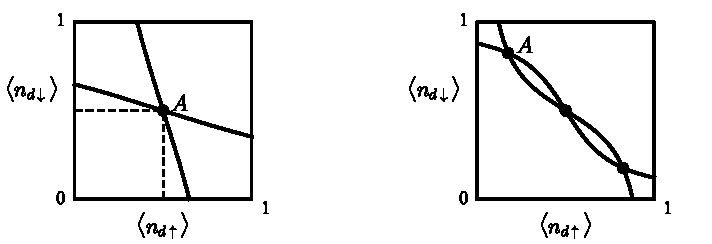
\includegraphics[width=9.5cm]{fig11-6.pdf}\\[0.3em]
{\small (a) $U=\Gamma$，$E_{\mathrm{F}}-E_{\mathrm{d}}=\dfrac{U}{2}$，
$\langle n_{\mathrm{d}\downarrow}\rangle=\langle n_{\mathrm{d}\uparrow}\rangle=\dfrac{1}{2}$
\qquad
(b) $U=5\Gamma$，$E_{\mathrm{F}}-E_{\mathrm{d}}=\dfrac{U}{2}$，
$\langle n_{\mathrm{d}\downarrow}\rangle\neq\langle n_{\mathrm{d}\uparrow}\rangle$}\\[0.2em]
{\small 图 11.6\quad $\langle n_{\mathrm{d}\sigma}\rangle$ 的自洽解}
\end{minipage}
\end{center}

\begin{center}
\begin{minipage}{6cm}
\centering
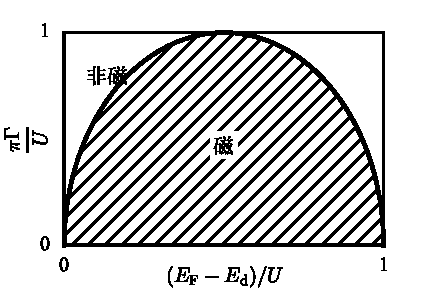
\includegraphics[width=6cm]{fig11-7.pdf}\\{\small 图 11.7\quad 安德逊哈特利-福克解的磁性与非磁性区域}
\end{minipage}
\end{center}

综上所述，安德逊模型的哈特利-福克近似解能够说明非磁性金属基体中杂质磁矩的形成条件.当费密能级 $E_{\mathrm{F}}$ 位于 $E_{\mathrm{d}}$ 和 $E_{\mathrm{d}}+U$ 的中间、并且d电子态密度的半峰宽 $\Gamma\ll U$ 时，将是形成局域磁矩的最有利条件.稀土元素的杂质（其 $U\approx15$ eV，$\Gamma\leqslant1$ eV）往往满足最有利条件，因此它们多数在金属中形成局域磁矩.由于铁族过渡元素的 $U\approx10$ eV，$\Gamma\approx2\sim5$ eV，其 $\pi\Gamma$ 值，对于不同的铁族元素，可能小于或大于U，而磁与非磁解的转变边界大约在 $\pi\Gamma/U=1$ 处.按此估计，当铁族杂质溶于金属中时有些产生局域磁矩，另一些则只能形成非磁性的局域态.在具体说明各种杂质的局域磁矩时，还需要考虑d能级简并问题，特别是各简并轨道间交换作用对边界的修正，这方面的工作可参阅文献[6].近年来安德逊模型已推广到每个元胞中均含一个磁性原子的情况，此即周期性安德逊模型（又称安德逊晶格模型，简称ALM），它用于说明稀土金属及其化合物的变价特性\textsuperscript{[7]}和重费密子特征.我们将在§7中引入ALM，并在§8中介绍此模型对重费密子系统的应用.

\section{s-d交换模型}

如果杂质原子在金属中已形成局域磁矩，它对金属中电子的输运特性有何影响？要回答这个问题必须首先讨论金属中局域磁矩与传导电子之间的相互作用.

设金属中含有少量磁性杂质原子，并都已形成磁矩，在 $\boldsymbol{R}_{n}$ 格点上杂质的自旋矩由算符 $\hat{\boldsymbol{S}}_{n}$ 描述，它代表杂质d壳层局域电子的总自旋算符.从多体理论可以证明传导电子(s)与形成磁矩的局域电子(d)之间的交换作用为
\begin{equation}
\begin{aligned}
  \mathscr{H}_{\mathrm{s}\text{-}\mathrm{d}}
  &=-\frac{J}{N}\sum_{n}\sum_{k,\,k'}
  \mathrm{e}^{\mathrm{i}(\boldsymbol{k}'-\boldsymbol{k})\cdot\boldsymbol{R}_{n}}
  \bigl\{\bigl(C^{+}_{k\uparrow}C_{k'\uparrow}
  -C^{+}_{k\downarrow}C_{k'\downarrow}\bigr)\hat{S}^{z}_{n}\\
  &\qquad+C^{+}_{k\uparrow}C_{k'\downarrow}\hat{S}^{-}_{n}
  +C^{+}_{k\downarrow}C_{k'\uparrow}\hat{S}^{+}_{n}\bigr\}
\end{aligned}
\end{equation}
称为s-d交换作用，其中J为交换积分，N代表原子数，$C^{+}_{k\sigma}$ 与 $C_{k\sigma}$（$\sigma=\uparrow,\,\downarrow$）是传导电子的产生和消灭算符，$\boldsymbol{k}$ 为波矢.式(11.3.1)就是局域磁矩与传导电子相互作用哈密顿量.

我们将介绍糟谷（Kasuya）的简单证明\textsuperscript{[8]}，讨论杂质自旋 $S_{n}=\dfrac{1}{2}$ 情况.由于存在杂质磁矩，应要求d态满足单占条件
\begin{equation}
  C^{+}_{n\uparrow}C_{n\uparrow}+C^{+}_{n\downarrow}C_{n\downarrow}=1
\end{equation}
这时d电子要么占据自旋朝上态，要么自旋朝下，从而保证 $S_{n}=\dfrac{1}{2}$.$C^{+}_{n\sigma}$ 与 $C_{n\sigma}$ 是局域电子(d)的产生及消灭算符.根据式(3.2.16)，$\hat{\boldsymbol{S}}_{n}$ 与 $C^{+}_{n\sigma}$、$C_{n\sigma}$ 的关系为
\begin{equation}
\left.
\begin{aligned}
  &\frac{1}{2}\bigl(C^{+}_{n\uparrow}C_{n\uparrow}
  -C^{+}_{n\downarrow}C_{n\downarrow}\bigr)=\hat{S}^{z}_{n}\\
  &C^{+}_{n\uparrow}C_{n\downarrow}=\hat{S}^{+}_{n}\\
  &C^{+}_{n\downarrow}C_{n\uparrow}=\hat{S}^{-}_{n}
\end{aligned}\right\}
\end{equation}
设 $\phi_{k}(\boldsymbol{r})$ 为传导电子(s)的布洛赫函数，$\phi_{\mathrm{L}}(\boldsymbol{r}-\boldsymbol{R}_{n})$ 代表以 $\boldsymbol{R}_{n}$ 格点为中心的局域d电子波函数，则s电子与d电子系统的二次量子化态矢量可写成
\begin{equation}
  \varPsi(\boldsymbol{r},\zeta)
  =\sum_{k,\,\sigma}C_{k\sigma}\phi_{k}(\boldsymbol{r})\chi_{\sigma}(\zeta)
  +\sum_{n,\,\sigma}C_{n\sigma}
  \phi_{\mathrm{L}}(\boldsymbol{r}-\boldsymbol{R}_{n})\chi_{\sigma}(\zeta)
\end{equation}
其中 $\chi_{\sigma}(\zeta)$ 为单电子的自旋函数，$\zeta$ 为自旋坐标，并满足条件：
\begin{equation}
  \int\chi^{+}_{\sigma}(\zeta)\chi_{\sigma'}(\zeta)\,\mathrm{d}\zeta
  =\delta_{\sigma\sigma'}
\end{equation}
系统的电子-电子相互作用可表示为
\begin{equation}
  \frac{1}{2}\int\cdots\int
  \varPsi^{+}(\boldsymbol{r}_{1},\zeta_{1})
  \varPsi^{+}(\boldsymbol{r}_{2},\zeta_{2})
  v(\boldsymbol{r}_{12})
  \varPsi(\boldsymbol{r}_{2},\zeta_{2})
  \varPsi(\boldsymbol{r}_{1},\zeta_{1})
  \,\mathrm{d}\boldsymbol{r}_{1}\,\mathrm{d}\boldsymbol{r}_{2}
  \,\mathrm{d}\zeta_{1}\,\mathrm{d}\zeta_{2}
\end{equation}
这里 $v(\boldsymbol{r}_{12})$ 为电子间的二体互作用势，而
\begin{equation}
  \boldsymbol{r}_{12}=\boldsymbol{r}_{1}-\boldsymbol{r}_{2}
\end{equation}
当式(11.3.4)代入式(11.3.6)后，将得到很多项.我们仅取其中含算符
$C^{+}_{k\sigma}C_{k'\sigma'}C^{+}_{n\sigma''}C_{n\sigma'''}$
的项 $\mathscr{H}_{i}$，它代表传导电子不改变局域电子位置的散射项.这样做才能代表传导电子与局域自旋的互作用.再考虑到互作用势 $v(\boldsymbol{r}_{12})$ 与自旋无关，这项作用应满足总自旋守恒条件，得到
\begin{equation}
\begin{aligned}
  \mathscr{H}_{i}&=\sum_{n}\sum_{k,\,k'}\sum_{\sigma,\,\sigma'}
  \bigl\{C^{+}_{k\sigma}C_{k'\sigma}C^{+}_{n\sigma'}C_{n\sigma'}
  \langle\,kn\mid v\mid k'n\,\rangle\\
  &\quad-C^{+}_{k\sigma}C_{k'\sigma'}C^{+}_{n\sigma'}C_{n\sigma}
  \langle\,kn\mid v\mid nk'\,\rangle\bigr\}
\end{aligned}
\end{equation}
这里
\begin{equation}
\begin{aligned}
  \langle\,kn\mid v\mid k'n\,\rangle
  &=\int\phi^{*}_{k}(\boldsymbol{r}_{1})
  \phi^{*}_{\mathrm{L}}(\boldsymbol{r}_{2}-\boldsymbol{R}_{n})
  v(\boldsymbol{r}_{12})\\
  &\qquad\times\phi_{k'}(\boldsymbol{r}_{1})
  \phi_{\mathrm{L}}(\boldsymbol{r}_{2}-\boldsymbol{R}_{n})
  \,\mathrm{d}\boldsymbol{r}_{1}\,\mathrm{d}\boldsymbol{r}_{2}
\end{aligned}
\end{equation}
代表库仑项，
\begin{equation}
\begin{aligned}
  \langle\,kn\mid v\mid nk'\,\rangle
  &=\int\phi^{*}_{k}(\boldsymbol{r}_{1})
  \phi^{*}_{\mathrm{L}}(\boldsymbol{r}_{2}-\boldsymbol{R}_{n})
  v(\boldsymbol{r}_{12})\\
  &\qquad\times\phi_{\mathrm{L}}(\boldsymbol{r}_{1}-\boldsymbol{R}_{n})
  \phi_{k'}(\boldsymbol{r}_{2})
  \,\mathrm{d}\boldsymbol{r}_{1}\,\mathrm{d}\boldsymbol{r}_{2}
\end{aligned}
\end{equation}
代表交换项.

将 $\mathscr{H}_{i}$ 中自旋朝上和朝下态具体写出，并将式(11.3.8)中两项适当归并和整理成
\begin{equation}
\begin{aligned}
  \mathscr{H}_{i}&=\sum_{n}\sum_{k,\,k'}
  \bigl\{\bigl(C^{+}_{k\uparrow}C_{k'\uparrow}
  +C^{+}_{k\downarrow}C_{k'\downarrow}\bigr)
  \bigl(C^{+}_{n\uparrow}C_{n\uparrow}
  +C^{+}_{n\downarrow}C_{n\downarrow}\bigr)\\
  &\qquad\times\bigl[\langle kn\mid v\mid k'n\rangle
  -\frac{1}{2}\langle kn\mid v\mid nk'\rangle\bigr]\bigr\}\\
  &\quad-\sum_{n}\sum_{k,\,k'}\bigl\{\bigl(C^{+}_{k\uparrow}C_{k'\uparrow}
  -C^{+}_{k\downarrow}C_{k'\downarrow}\bigr)
  \frac{1}{2}\bigl(C^{+}_{n\uparrow}C_{n\uparrow}
  -C^{+}_{n\downarrow}C_{n\downarrow}\bigr)\\
  &\qquad+\bigl(C^{+}_{k\uparrow}C_{k'\downarrow}C^{+}_{n\downarrow}C_{n\uparrow}
  +C^{+}_{k\downarrow}C_{k'\uparrow}C^{+}_{n\uparrow}C_{n\downarrow}\bigr)\bigr\}
  \langle kn\mid v\mid nk'\rangle
\end{aligned}
\end{equation}
再将d电子的单占条件和关系式(11.3.3)代入，则上式可写为局域自旋 $\hat{\boldsymbol{S}}_{n}$ 与传导电子的互作用
\begin{equation}
\begin{aligned}
  \mathscr{H}_{i}&=\sum_{n}\sum_{k,\,k'}
  \bigl\{\bigl(C^{+}_{k\uparrow}C_{k'\uparrow}
  +C^{+}_{k\downarrow}C_{k'\downarrow}\bigr)
  \bigl[\langle kn\mid v\mid k'n\rangle\\
  &\qquad-\frac{1}{2}\langle kn\mid v\mid nk'\rangle\bigr]\bigr\}
  -\sum_{n}\sum_{k,\,k'}\bigl\{\bigl(C^{+}_{k\uparrow}C_{k'\uparrow}
  -C^{+}_{k\downarrow}C_{k'\downarrow}\bigr)\hat{S}^{z}_{n}\\
  &\qquad+C^{+}_{k\uparrow}C_{k'\downarrow}\hat{S}^{-}_{n}
  +C^{+}_{k\downarrow}C_{k'\uparrow}\hat{S}^{+}_{n}\bigr\}
  \langle kn\mid v\mid nk'\rangle
\end{aligned}
\end{equation}
现在，具体分析库仑项 $\langle kn\mid v\mid k'n\rangle$ 及交换项 $\langle kn\mid v\mid nk'\rangle$.先看交换项，利用布洛赫定理
\begin{equation}
  \phi_{k}(\boldsymbol{r})=\mathrm{e}^{\mathrm{i}\boldsymbol{k}\cdot\boldsymbol{R}_{n}}
  \phi_{k}(\boldsymbol{r}-\boldsymbol{R}_{n})
\end{equation}
将交换项式(11.3.10)改写成
\begin{equation}
\begin{aligned}
  \langle\,kn\mid v\mid nk'\,\rangle
  &=\mathrm{e}^{\mathrm{i}(\boldsymbol{k}'-\boldsymbol{k})\cdot\boldsymbol{R}_{n}}
  \int\!\!\int\phi^{*}_{k}(\boldsymbol{r}_{1})
  \phi^{*}_{\mathrm{L}}(\boldsymbol{r}_{2})\\
  &\qquad\times v(\boldsymbol{r}_{12})
  \phi_{\mathrm{L}}(\boldsymbol{r}_{1})\phi_{k'}(\boldsymbol{r}_{2})
  \,\mathrm{d}\boldsymbol{r}_{1}\,\mathrm{d}\boldsymbol{r}_{2}
\end{aligned}
\end{equation}
再将布洛赫函数 $\phi_{k}(\boldsymbol{r})$ 用瓦尼尔函数 $a(\boldsymbol{r}-\boldsymbol{R}_{j})$ 表示，作变换
\begin{equation}
  \phi_{k}(\boldsymbol{r})=\frac{1}{\sqrt{N}}\sum_{j}
  \mathrm{e}^{\mathrm{i}\boldsymbol{k}\cdot\boldsymbol{R}_{j}}
  a(\boldsymbol{r}-\boldsymbol{R}_{j})
\end{equation}
得到交换项的局域函数表示式：
\begin{equation}
\begin{aligned}
  \langle\,kn\mid v\mid nk'\,\rangle
  &=\frac{1}{N}\mathrm{e}^{\mathrm{i}(\boldsymbol{k}'-\boldsymbol{k})\cdot\boldsymbol{R}_{n}}
  \sum_{ij}\mathrm{e}^{\mathrm{i}(\boldsymbol{k}'\cdot\boldsymbol{R}_{j}
  -\boldsymbol{k}\cdot\boldsymbol{R}_{i})}\\
  &\qquad\times\int\!\!\int a^{*}(\boldsymbol{r}_{1}-\boldsymbol{R}_{i})
  \phi^{*}_{\mathrm{L}}(\boldsymbol{r}_{2})v(\boldsymbol{r}_{12})
  \phi_{\mathrm{L}}(\boldsymbol{r}_{1})
  a(\boldsymbol{r}_{2}-\boldsymbol{R}_{j})
  \,\mathrm{d}\boldsymbol{r}_{1}\,\mathrm{d}\boldsymbol{r}_{2}
\end{aligned}
\end{equation}
由于 $\boldsymbol{R}_{i}=\boldsymbol{R}_{j}=0$ 项对积分贡献最大，上式可近似为
\begin{equation}
  \langle\,kn\mid v\mid nk'\,\rangle
  \approx\frac{1}{N}\mathrm{e}^{\mathrm{i}(\boldsymbol{k}'-\boldsymbol{k})\cdot\boldsymbol{R}_{n}}J
\end{equation}
\begin{equation}
  J=\int\!\!\int a^{*}(\boldsymbol{r}_{1})
  \phi^{*}_{\mathrm{L}}(\boldsymbol{r}_{2})v(\boldsymbol{r}_{12})
  \phi_{\mathrm{L}}(\boldsymbol{r}_{1})a(\boldsymbol{r}_{2})
  \,\mathrm{d}\boldsymbol{r}_{1}\,\mathrm{d}\boldsymbol{r}_{2}
\end{equation}
为常数，代表同一格点周围s电子与d电子的交换积分.在同样的近似下可将库仑项表示为
\begin{equation}
  \langle\,kn\mid v\mid k'n\,\rangle
  \approx\frac{1}{N}\mathrm{e}^{\mathrm{i}(\boldsymbol{k}'-\boldsymbol{k})\cdot\boldsymbol{R}_{n}}U
\end{equation}
其中
\begin{equation}
  U\equiv\int\!\!\int a^{*}(\boldsymbol{r}_{1})
  \phi^{*}_{\mathrm{L}}(\boldsymbol{r}_{2})v(\boldsymbol{r}_{12})
  a(\boldsymbol{r}_{1})\phi_{\mathrm{L}}(\boldsymbol{r}_{2})
  \,\mathrm{d}\boldsymbol{r}_{1}\,\mathrm{d}\boldsymbol{r}_{2}
\end{equation}
定义 $V\equiv U-\dfrac{1}{2}J$，并将式(11.3.17)和(11.3.19)式代入式(11.3.12)，求得
\begin{equation}
\begin{aligned}
  \mathscr{H}_{i}&=\frac{V}{N}\sum_{n}\sum_{k,\,k'}
  \mathrm{e}^{\mathrm{i}(\boldsymbol{k}'-\boldsymbol{k})\cdot\boldsymbol{R}_{n}}
  \bigl(C^{+}_{k\uparrow}C_{k'\uparrow}
  +C^{+}_{k\downarrow}C_{k'\downarrow}\bigr)\\
  &\quad-\frac{J}{N}\sum_{n}\sum_{k,\,k'}
  \mathrm{e}^{\mathrm{i}(\boldsymbol{k}'-\boldsymbol{k})\cdot\boldsymbol{R}_{n}}
  \bigl\{\bigl(C^{+}_{k\uparrow}C_{k'\uparrow}
  -C^{+}_{k\downarrow}C_{k'\downarrow}\bigr)\hat{S}^{z}_{n}\\
  &\qquad+C^{+}_{k\uparrow}C_{k'\downarrow}\hat{S}^{-}_{n}
  +C^{+}_{k\downarrow}C_{k'\uparrow}\hat{S}^{+}_{n}\bigr\}
\end{aligned}
\end{equation}
其中第一个求和项是与杂质自旋无关的散射项，容易证明它是 $\delta$ 型单子势能
\begin{equation*}
  \frac{V}{N}\sum_{n}\delta(\boldsymbol{r}-\boldsymbol{R}_{n})
\end{equation*}
的二次量子化表示式，代表杂质破坏晶格周期性所提供的势散射项.式(11.3.21)中第二个求和项正好是式(11.3.1)给出的s-d交换作用 $\mathscr{H}_{\mathrm{s}\text{-}\mathrm{d}}$.

略去与自旋无关的势散射项，再加入金属中传导电子哈密顿量
$\mathscr{H}_{0}=\sum_{k,\,\sigma}\varepsilon_{k}C^{+}_{k\sigma}C_{k\sigma}$，
得到系统的总哈密顿量：
\begin{equation}
\begin{aligned}
  \mathscr{H}&=\mathscr{H}_{0}+\mathscr{H}_{\mathrm{s}\text{-}\mathrm{d}}
  =\sum_{k,\,\sigma}\varepsilon_{k}C^{+}_{k\sigma}C_{k\sigma}\\
  &\quad-\frac{J}{N}\sum_{n}\sum_{k,\,k'}
  \mathrm{e}^{\mathrm{i}(\boldsymbol{k}'-\boldsymbol{k})\cdot\boldsymbol{R}_{n}}
  \bigl\{\bigl(C^{+}_{k\uparrow}C_{k'\uparrow}
  -C^{+}_{k\downarrow}C_{k'\downarrow}\bigr)\hat{S}^{z}_{n}\\
  &\qquad+C^{+}_{k\uparrow}C_{k'\downarrow}\hat{S}^{-}_{n}
  +C^{+}_{k\downarrow}C_{k'\uparrow}\hat{S}^{+}_{n}\bigr\}
\end{aligned}
\end{equation}
其中 $\varepsilon_{k}$ 代表从费密能级 $E_{\mathrm{F}}$ 算起的能带电子能量，这就是s-d模型的哈密顿量.

引入泡利矩阵
\begin{equation}
  \hat{\sigma}^{z}=\begin{pmatrix}1&0\\0&-1\end{pmatrix},
  \quad
  \hat{\sigma}^{+}=\begin{pmatrix}0&2\\0&0\end{pmatrix},
  \quad
  \hat{\sigma}^{-}=\begin{pmatrix}0&0\\2&0\end{pmatrix}
\end{equation}
并利用关系式
\begin{equation}
  \hat{\boldsymbol{S}}\cdot\hat{\boldsymbol{\sigma}}
  =\hat{S}^{z}\hat{\sigma}^{z}
  +\frac{1}{2}\bigl(\hat{S}^{+}\hat{\sigma}^{-}
  +\hat{S}^{-}\hat{\sigma}^{+}\bigr)
\end{equation}
可将s-d互作用式(11.3.21)改写成
\begin{equation}
  \mathscr{H}_{\mathrm{s}\text{-}\mathrm{d}}
  =-\frac{J}{N}\sum_{n}\sum_{k,\,k'}\sum_{\mu,\,\mu'}
  \mathrm{e}^{\mathrm{i}(\boldsymbol{k}'-\boldsymbol{k})\cdot\boldsymbol{R}_{n}}\,
  \hat{\boldsymbol{S}}_{n}\cdot\hat{\boldsymbol{\sigma}}_{\mu\mu'}\,
  C^{+}_{k\mu}C_{k'\mu'}
\end{equation}
这里用 $\mu$、$\mu'$ 代表电子自旋取向.式(11.3.25)所对应的单电子势能为
\begin{equation}
  -\frac{J}{N}\sum_{n}
  \bigl(\hat{\boldsymbol{S}}_{n}\cdot\hat{\boldsymbol{\sigma}}\bigr)
  \delta(\boldsymbol{r}-\boldsymbol{R}_{n})
\end{equation}
上式说明s-d互作用是局域自旋 $\hat{\boldsymbol{S}}_{n}$ 与传导电子泡利自旋 $\hat{\boldsymbol{\sigma}}$ 之间的短程交换作用.

\section{RKKY互作用}

为了研究磁性金属及合金中的磁序，必须讨论局域磁矩之间的相互耦合问题.茹德曼（Ruderman）、基泰尔（Kittel）\textsuperscript{[9]}、芳田奎（Yosida）\textsuperscript{[10]}以及糟谷\textsuperscript{[8]}等人的研究指出，局域磁矩通过传导电子所产生的间接交换作用可写成下列形式.
\begin{equation}
  \mathscr{H}_{\mathrm{RKKY}}
  ={\sum_{n,\,m}}'\hat{\boldsymbol{S}}_{n}\cdot\hat{\boldsymbol{S}}_{m}\,
  \mathscr{J}(|\boldsymbol{R}_{n}-\boldsymbol{R}_{m}|)
\end{equation}
其中互作用强度
\begin{equation}
  \mathscr{J}(|\boldsymbol{R}|)=\frac{9\pi}{2}
  \biggl(\frac{J^{2}}{E_{\mathrm{F}}}\biggr)
  \biggl\{\frac{\cos 2k_{\mathrm{F}}R}{(2k_{\mathrm{F}}R)^{3}}
  -\frac{\sin 2k_{\mathrm{F}}R}{(2k_{\mathrm{F}}R)^{4}}\biggr\}
\end{equation}
这是一个振荡型的相互作用，并具有长程特性：当R较大时，交换作用强度 $\mathscr{J}(|\boldsymbol{R}|)$ 按 $R^{-3}$ 衰减，并以 $(2k_{\mathrm{F}})^{-1}$ 为周期振荡，表现出不同于海森伯交换作用的特征，通常称为RKKY互作用.

由于RKKY互作用随距离增大振荡，交换作用强度 $\mathscr{J}(|\boldsymbol{R}|)$ 将改变符号，这一特征对于稀土金属、磁性合金的磁序结构有重要影响.RKKY互作用可以预言各种复杂磁序结构的存在，包括螺旋磁结构\textsuperscript{[11]}，还成功地应用于磁性半导体\textsuperscript{[12]}.

RKKY互作用可由s-d交换作用导出，其作法与第五章§5中推导电子间通过声子的间接互作用相似.我们可以利用二级微扰处理s-d互作用，并只对传导电子态平均，从而消去电子算符求得局域磁矩通过传导电子的有效互作用\textsuperscript{[13]}
\begin{equation}
  \mathscr{H}_{\mathrm{eff}}=\sum'_{k,\,k'}\sum_{\mu,\,\mu'}
  \frac{\langle\,k\mu\mid\mathscr{H}_{\mathrm{s}\text{-}\mathrm{d}}\mid k'\mu'\,\rangle
  \langle\,k'\mu'\mid\mathscr{H}_{\mathrm{s}\text{-}\mathrm{d}}\mid k\mu\,\rangle}
  {\varepsilon_{k}-\varepsilon_{k'}}
\end{equation}
$|k\mu\rangle$ 代表布洛赫电子状态.将式(11.3.25)的 $\mathscr{H}_{\mathrm{s}\text{-}\mathrm{d}}$ 代入上式，并计算电子态平均，求得
\begin{equation}
\begin{aligned}
  \mathscr{H}_{\mathrm{eff}}
  &=\biggl(\frac{J}{N}\biggr)^{2}\sum_{n,\,m}\sum_{k,\,k'}\sum_{\mu,\,\mu'}
  \mathrm{e}^{\mathrm{i}(\boldsymbol{k}'-\boldsymbol{k})\cdot(\boldsymbol{R}_{n}-\boldsymbol{R}_{m})}
  f_{k}(1-f_{k'})\\
  &\qquad\times\frac{(\hat{\boldsymbol{S}}_{n}\cdot\hat{\boldsymbol{\sigma}}_{\mu\mu'})
  (\hat{\boldsymbol{S}}_{m}\cdot\hat{\boldsymbol{\sigma}}_{\mu'\mu})}
  {\varepsilon_{k}-\varepsilon_{k'}}
\end{aligned}
\end{equation}
其中 $f_{k}$ 为零温时传导电子的费密分布函数，而算符部分可用矩阵迹表示
\begin{equation}
  \sum_{\mu,\,\mu'}
  (\hat{\boldsymbol{S}}_{n}\cdot\hat{\boldsymbol{\sigma}}_{\mu\mu'})
  (\hat{\boldsymbol{S}}_{m}\cdot\hat{\boldsymbol{\sigma}}_{\mu'\mu})
  =\mathrm{Tr}\{(\hat{\boldsymbol{\sigma}}\cdot\hat{\boldsymbol{S}}_{n})
  (\hat{\boldsymbol{\sigma}}\cdot\hat{\boldsymbol{S}}_{m})\}
\end{equation}
由于 $\hat{\boldsymbol{\sigma}}$ 与 $\hat{\boldsymbol{S}}_{n}$、$\hat{\boldsymbol{S}}_{m}$ 可对易，存在下列等式\textsuperscript{[14]}：
\begin{equation}
  (\hat{\boldsymbol{\sigma}}\cdot\hat{\boldsymbol{S}}_{n})
  (\hat{\boldsymbol{\sigma}}\cdot\hat{\boldsymbol{S}}_{m})
  =\hat{\boldsymbol{S}}_{n}\cdot\hat{\boldsymbol{S}}_{m}
  +\mathrm{i}\,\hat{\boldsymbol{\sigma}}\cdot
  (\hat{\boldsymbol{S}}_{n}\times\hat{\boldsymbol{S}}_{m})
\end{equation}
考虑到泡利矩阵之迹为零，因此式(11.4.6)中只有 $(\hat{\boldsymbol{S}}_{n}\cdot\hat{\boldsymbol{S}}_{m})$ 项对 $\mathscr{H}_{\mathrm{eff}}$ 的贡献
\begin{equation}
  \mathscr{H}_{\mathrm{eff}}
  =\sum_{n,\,m}(\hat{\boldsymbol{S}}_{n}\cdot\hat{\boldsymbol{S}}_{m})
  \biggl(\frac{J}{N}\biggr)^{2}\sum_{k,\,k'}
  \frac{\mathrm{e}^{\mathrm{i}(\boldsymbol{k}'-\boldsymbol{k})\cdot(\boldsymbol{R}_{n}-\boldsymbol{R}_{m})}}
  {\varepsilon_{k}-\varepsilon_{k'}}
  f_{k}(1-f_{k'})
\end{equation}
$\mathscr{H}_{\mathrm{eff}}$ 中 $n=m$ 项，由于有算符等式
\begin{equation}
  (\hat{\boldsymbol{S}}\cdot\hat{\boldsymbol{S}})=S(S+1)
\end{equation}
可写成
\begin{equation}
  \biggl\{\biggl(\frac{J}{N}\biggr)^{2}
  \sum_{k<k_{\mathrm{F}}}\sum_{k'>k_{\mathrm{F}}}
  \frac{1}{\varepsilon_{k}-\varepsilon_{k'}}\biggr\}
  \sum_{n}S_{n}(S_{n}+1)
\end{equation}
它仅代表s-d互作用对电子自能的修正，而 $n\neq m$ 部分才是局域磁矩通过传导电子的间接交换作用，因此RKKY互作用为
\begin{equation}
  \mathscr{H}_{\mathrm{RKKY}}
  ={\sum_{n,\,m}}'(\hat{\boldsymbol{S}}_{n}\cdot\hat{\boldsymbol{S}}_{m})\,
  \mathscr{J}(|\boldsymbol{R}_{n}-\boldsymbol{R}_{m}|)
\end{equation}
其中
\begin{equation}
\begin{aligned}
  \mathscr{J}(|\boldsymbol{R}|)
  &=\biggl(\frac{J}{N}\biggr)^{2}{\sum_{k,\,k'}}'
  \frac{\mathrm{e}^{\mathrm{i}(\boldsymbol{k}'-\boldsymbol{k})\cdot\boldsymbol{R}}}
  {\varepsilon_{k}-\varepsilon_{k'}}f_{k}(1-f_{k'})\\
  &=\biggl(\frac{J}{N}\biggr)^{2}
  \sum_{k<k_{\mathrm{F}}}\sum_{k'>k_{\mathrm{F}}}
  \frac{\mathrm{e}^{\mathrm{i}(\boldsymbol{k}'-\boldsymbol{k})\cdot\boldsymbol{R}}}
  {\varepsilon_{k}-\varepsilon_{k'}}\\
  &=\biggl(\frac{J}{N}\biggr)^{2}\frac{V^{2}}{(2\pi)^{6}}\frac{2m}{\hbar^{2}}
  \mathscr{P}\!\int_{k<k_{\mathrm{F}}}\mathrm{d}^{3}k
  \int_{k'>k_{\mathrm{F}}}\mathrm{d}^{3}k'\,
  \frac{\mathrm{e}^{\mathrm{i}(\boldsymbol{k}'-\boldsymbol{k})\cdot\boldsymbol{R}}}
  {k^{2}-k'^{2}}
\end{aligned}
\end{equation}
范夫累克（van Vleck）\textsuperscript{[15]}曾经计算了这个主值积分，其结果为
\begin{equation}
  \mathscr{J}(|\boldsymbol{R}|)=\frac{9\pi}{2}\frac{J^{2}}{E_{\mathrm{F}}}
  F(2k_{\mathrm{F}}R)
\end{equation}
\begin{equation}
  F(x)=\frac{x\cos x-\sin x}{x^{4}}
\end{equation}
这就是推导RKKY互作用的主要步骤.近年来两局域磁矩间的RKKY互作用理论已被推广用于两铁磁金属层(FM)被非磁金属夹层(NM)隔开的FM-NM-FM金属磁多层结构，涉及巨磁电阻研究，并成功地解释了层间交换作用随夹层厚度改变的振荡特征\textsuperscript{[16]}.

\section{\texorpdfstring{近藤效应\textsuperscript{[17]}}{近藤效应[17]}}

在非磁性的简单金属（如Cu、Ag、Au等）中掺入微量d壳层未填满的磁性杂质（如Fe、Mn、Mo、Os等）后就形成了稀磁合金.在稀磁合金中普遍观测到低温电阻极小现象，其示意图如图11.8中实线所示.对于多数材料，电阻极小点出现在10～20K温区内.若从电阻曲线中扣除电子被热声子散射的电阻 $R_{\text{声子}}=AT^{5}$ 贡献后，得到磁性杂质对电阻的贡献随温度降低而增大，在电阻极小点附近实验数据可归纳成
\begin{equation}
  R_{\text{杂质}}=a-b\ln T
\end{equation}
表现出随温度降低按对数式规律增长的特征，与通常非磁杂质的剩余电阻（与温度无关）规律迥然不同.实验还证实，只要测得了电阻极小，必能同时测出金属中有局域杂质磁矩存在，说明电阻极小现象是杂质磁矩所造成的.1964年近藤（Kondo）\textsuperscript{[18]}指出，必须用s-d交换模型处理问题.当电子被磁杂质散射时，不仅电子的自旋状态发生变化，同时杂质本身的自旋状态也要发生相应的变化，这是一种多粒子效应.近藤用多体理论对电子-磁杂质散射问题作微扰计算，很自然地求得了杂质电阻随温度降低的对数式增长规律，解释了电阻极小现象.

\begin{center}
\begin{minipage}{5.5cm}
\centering
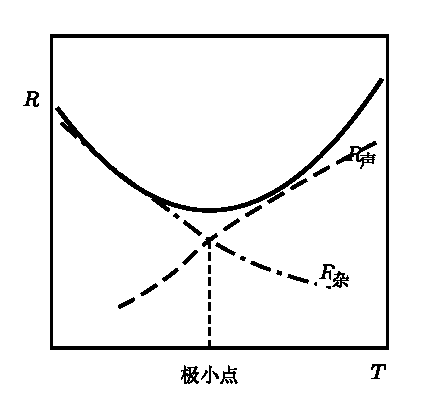
\includegraphics[width=5.5cm]{fig11-8.pdf}\\[0.3em]
{\small （$R=R_{\text{声子}}+R_{\text{杂质}}$）}\\[0.2em]
{\small 图 11.8\quad 电阻极小示意图}
\end{minipage}
\end{center}

\subsection*{1. 近藤的工作}

由于电阻极小现象可以在杂质浓度非常低的情况下被观察到（杂质原子浓度小于 $10^{-4}\%$），因此电阻极小是孤立磁杂质与传导电子间相互作用特征的反映，而不是磁杂质之间相互作用所造成的.近藤采用单个磁性杂质与传导电子之间的s-d交换模型描述稀磁合金的问题，他假定磁性杂质位于原点，具有确定的自旋S，则根据式(11.3.1)、(11.3.22)和(11.3.25)系统的总哈密顿量为
\begin{equation}
  \mathscr{H}=\sum_{k,\,\mu}\varepsilon_{k}C^{+}_{k\mu}C_{k\mu}
  -\biggl(\frac{J}{N}\biggr)\sum_{k,\,k'}\sum_{\mu,\,\mu'}
  \hat{\boldsymbol{S}}\cdot\hat{\boldsymbol{\sigma}}_{\mu\mu'}\,
  C^{+}_{k\mu}C_{k'\mu'}
\end{equation}
式(11.5.2)又称近藤哈密顿量.其中s-d交换作用部分
\begin{equation}
  \mathscr{H}_{\mathrm{s}\text{-}\mathrm{d}}
  =-\biggl(\frac{J}{N}\biggr)\sum_{k,\,k'}\sum_{\mu,\,\mu'}
  \Bigl\{\hat{S}^{z}\hat{\sigma}^{z}_{\mu\mu'}
  +\frac{1}{2}\hat{S}^{+}\hat{\sigma}^{-}_{\mu\mu'}
  +\frac{1}{2}\hat{S}^{-}\hat{\sigma}^{+}_{\mu\mu'}\Bigr\}
  C^{+}_{k\mu}C_{k'\mu'}
\end{equation}
由于 $\hat{S}^{\pm}$ 代表杂质自旋上升及下降算符，$\hat{\sigma}^{\pm}$ 描述传导电子的自旋上升及下降.因此，式(11.5.3)中第一项为非自旋倒逆（non spin-flip）互作用，第二、三项是自旋倒逆（spin-flip）部分，它们涉及电子自旋上升（或下降）与杂质自旋下降（或上升）同时发生的散射过程，因为耦合常数的绝对值 $|J|$ 一般比传导电子的费密能 $E_{\mathrm{F}}$ 小得多，所以近藤最初的计算是用微扰论作出的.他讨论了电子从初态 $(\boldsymbol{k},\mu)$ 散射到终态 $(\boldsymbol{k}',\mu')$，同时杂质自旋从 $\alpha$ 态变为 $\alpha'$ 态的散射概率.在一级近似下，跃迁矩阵元为
\begin{equation}
  T^{(1)}_{\mu'\alpha',\,\mu\alpha}
  =-\biggl(\frac{J}{N}\biggr)\hat{\boldsymbol{\sigma}}_{\mu'\mu}
  \cdot\hat{\boldsymbol{S}}_{\alpha'\alpha}
\end{equation}
$T^{(1)}$ 又称一级散射振幅.这里涉及电子自旋从 $\mu$ 变为 $\mu'$ 的下列4种过程：
\begin{equation}
\left.
\begin{aligned}
  &(\boldsymbol{k}\uparrow)\to(\boldsymbol{k}'\uparrow);
  \ (\boldsymbol{k}\downarrow)\to(\boldsymbol{k}'\downarrow)\\
  &(\boldsymbol{k}\uparrow)\to(\boldsymbol{k}'\downarrow);
  \ (\boldsymbol{k}\downarrow)\to(\boldsymbol{k}'\uparrow)
\end{aligned}\right\}
\end{equation}
相应的 $T^{(1)}$ 分别为
\begin{equation}
  \mp\biggl(\frac{J}{N}\biggr)\hat{S}^{z},
  \qquad \biggl(\frac{J}{N}\biggr)\hat{S}^{\pm}
\end{equation}
因此，由 $T^{(1)}$ 模的平方求出的玻恩近似散射概率正比于
\begin{equation}
  J^{2}\biggl\{(\hat{S}^{z})^{2}
  +\frac{1}{2}\bigl(\hat{S}^{+}\hat{S}^{-}
  +\hat{S}^{-}\hat{S}^{+}\bigr)\biggr\}
  =J^{2}S(S+1)
\end{equation}
是和温度无关的项，只能给出剩余电阻
\begin{equation}
  R_{0}=AJ^{2}S(S+1)
\end{equation}
式(11.5.8)与 $R_{\text{声子}}$ 组合不能说明电阻极小.显然，更重要的过程应当出现在散射振幅（即散射矩阵）的高阶近似中，对于二级微扰过程，散射要通过中间状态 $(\boldsymbol{k}'',\mu'')$ 进行.这里应当区分两种情况，(i)在 $(\boldsymbol{k}'',\mu'')$ 中间态上未被电子占据；(ii)已被电子占据.若以从 $(\boldsymbol{k}\downarrow)$ 态到 $(\boldsymbol{k}'\downarrow)$ 态经历自旋倒逆中间散射过程为例，则对于情况(i)由图11.9(a)描述，称为电子中间态过程.因为，$(\boldsymbol{k}\downarrow)$ 电子先跃迁到 $(\boldsymbol{k}''\uparrow)$ 态，然后再跃迁到 $(\boldsymbol{k}'\downarrow)$ 状态，而杂质自旋则经历先下降后上升的变化 $\hat{S}^{+}\hat{S}^{-}$，考虑到中间态电子处于热平衡，因此在 $(\boldsymbol{k}''\uparrow)$ 状态上未被占据概率应等于 $(1-f_{k''})$，$f_{k''}$ 为费密分布函数.于是求得电子中间态过程的二级散射振幅为
\begin{equation}
  \biggl(\frac{J}{N}\biggr)^{2}\sum_{k''}
  \frac{\hat{S}^{+}\hat{S}^{-}}{\varepsilon_{k}-\varepsilon_{k''}}
  (1-f_{k''})
\end{equation}
对于情况(ii)由图11.9(b)描述，属于空穴中间态过程.因为，要先从 $(\boldsymbol{k}''\uparrow)$ 状态上将电子激发到终态 $(\boldsymbol{k}'\downarrow)$，在 $(\boldsymbol{k}''\uparrow)$ 态则留下空穴，然后初态 $(\boldsymbol{k}\downarrow)$ 电子再与中间态 $(\boldsymbol{k}''\uparrow)$ 的空穴复合，因此电子自旋为先下降后上升，相应的杂质自旋则应经历先上升后下降的变化 $\hat{S}^{-}\hat{S}^{+}$，而且由于 $(\boldsymbol{k}''\uparrow)$ 态在热平衡时被占据概率是 $f_{k''}$，所以空穴中间态过程的二级散射振幅为
\begin{equation}
  \biggl(\frac{J}{N}\biggr)^{2}\sum_{k''}
  \frac{\hat{S}^{-}\hat{S}^{+}}{\varepsilon_{k}-\varepsilon_{k''}}f_{k''}
\end{equation}

\begin{center}
\begin{minipage}{9cm}
\centering
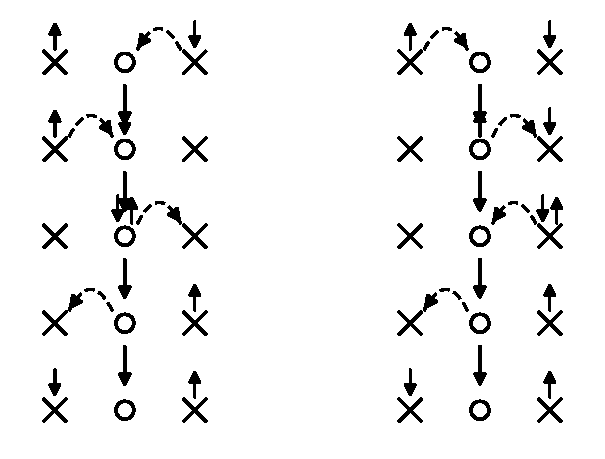
\includegraphics[width=9cm]{fig11-9.pdf}\\[0.3em]
{\small (a) 电子中间态\qquad\qquad (b) 空穴中间态}\\[0.2em]
{\small 图 11.9\quad 自旋倒逆散射的二级过程}
\end{minipage}
\end{center}

以上是s-d互作用中自旋倒逆部分
$\dfrac{1}{2}(\hat{S}^{+}\hat{\sigma}^{-}+\hat{S}^{-}\hat{\sigma}^{+})$
的贡献.对于非自旋倒逆互作用 $\hat{S}^{z}\hat{\sigma}^{z}$ 部分，只需将式(11.5.9)和式(11.5.10)中 $\hat{S}^{+}$ 和 $\hat{S}^{-}$ 用 $\hat{S}^{z}$ 代替，因此求得总的二级散射振幅
\begin{equation}
\begin{aligned}
  T^{(2)}_{\mu'\alpha',\,\mu\alpha}(\varepsilon)
  &=\biggl(\frac{J}{N}\biggr)^{2}\sum_{k''}
  \biggl\{\frac{(\hat{S}^{z})^{2}+\hat{S}^{+}\hat{S}^{-}}
  {\varepsilon-\varepsilon_{k''}}(1-f_{k''})
  +\frac{(\hat{S}^{z})^{2}+\hat{S}^{-}\hat{S}^{+}}
  {\varepsilon-\varepsilon_{k''}}f_{k''}\biggr\}\\
  &=\biggl(\frac{J}{N}\biggr)^{2}\sum_{k''}
  \biggl\{\frac{(\hat{S}^{z})^{2}+\hat{S}^{+}\hat{S}^{-}}
  {\varepsilon-\varepsilon_{k''}}
  -[\hat{S}^{+},\hat{S}^{-}]\frac{f_{k''}}{\varepsilon-\varepsilon_{k''}}\biggr\}
\end{aligned}
\end{equation}
式(11.5.11)后一等式右边第一项主要为非自旋倒逆过程的二级贡献，它仍是与温度无关的.第二项代表自旋倒逆过程的贡献，由于杂质的量子自旋算符具有如下特征：
\begin{equation}
  [\hat{S}^{+},\hat{S}^{-}]
  =\hat{S}^{+}\hat{S}^{-}-\hat{S}^{-}\hat{S}^{+}
  =2\hat{S}^{z}\neq0
\end{equation}
就得到含有温度因子
\begin{equation*}
  f_{k''}=\biggl[\exp\biggl(\frac{\varepsilon_{k''}}{k_{\mathrm{B}}T}\biggr)+1\biggr]^{-1}
\end{equation*}
的散射振幅项.

由于电阻极小是稀磁合金中的普遍现象，具体能带结构对它影响不大，可以采用简化态密度
\begin{equation}
  \rho(\varepsilon)=
  \begin{cases}
    N\rho_{\mathrm{F}} & (\text{当}\ |\varepsilon|<D\ \text{时})\\
    0 & (\text{当}\ |\varepsilon|>D\ \text{时})
  \end{cases}
\end{equation}
其中 $\rho_{\mathrm{F}}$ 代表平均每个电子在费密面上态密度，D代表导带的半宽度.对于能带半填满的金属，D近似等于费密能 $E_{\mathrm{F}}$.

不难计算出下列求和近似为
\begin{equation}
\begin{aligned}
  \biggl(\frac{J}{N}\biggr)\sum_{k''}\frac{f_{k''}}{\varepsilon-\varepsilon_{k''}}
  &\approx J\rho_{\mathrm{F}}\ln
  \frac{\sqrt{\varepsilon^{2}+(k_{\mathrm{B}}T)^{2}}}{E_{\mathrm{F}}}\\
  &=\begin{cases}
    J\rho_{\mathrm{F}}\ln\biggl(\dfrac{k_{\mathrm{B}}T}{D}\biggr)
    & (\text{当}\ \varepsilon=0\ \text{时})\\[0.8em]
    J\rho_{\mathrm{F}}\ln\biggl(\dfrac{|\varepsilon|}{D}\biggr)
    & (\text{当}\ T=0\ \text{K 时})
  \end{cases}
\end{aligned}
\end{equation}
式(11.5.14)表现出对数型的能量及温度函数特征.这正是所希望的，因为总的杂质电阻应该正比于费密面上 $(\varepsilon=0$ 处$)$ 电子被杂质散射的概率，即正比于总散射振幅的模方 $|T^{(1)}+T^{(2)}|^{2}$，其中交叉项提供正比于
\begin{equation}
  J^{3}\rho_{\mathrm{F}}\ln\biggl(\frac{k_{\mathrm{B}}T}{D}\biggr)
\end{equation}
的因子，所以一般说在耦合常数J的3次方项会出现 $\ln T$ 型式的温度因子.近藤\textsuperscript{[18]}算得的磁性杂质电阻为
\begin{equation}
  R_{\text{杂质}}=R_{0}\biggl\{1+4J\rho_{\mathrm{F}}
  \ln\biggl(\frac{k_{\mathrm{B}}T}{D}\biggr)+\cdots\biggr\}
\end{equation}
式(11.5.16)对于 $J>0$ 情况（称铁磁型s-d耦合），只给出随温度降低而减小的杂质电阻，它与热声子电阻 $R_{\text{声子}}$ 的温度变化趋势一致，因此 $J>0$ 情况不导致电阻极小.但是，对于 $J<0$ 情况（称反铁磁型s-d耦合），式(11.5.16)给出 $R_{\text{杂质}}=a-b\ln T$ 项，是随温度降低对数式增长的杂质电阻，它与热声子电阻 $AT^{5}$ 组合正好能说明电阻极小，多数稀磁合金属于 $J<0$ 的材料，因此电阻极小现象普遍能观察到，这些都是近藤计算的成功之处.

\subsection*{2. 近藤效应}

近藤的工作促进了实验工作者对稀磁合金低温特性的进一步研究，发现除电阻极小现象（又称电阻反常）外，还有磁化率、比热容等一系列低温反常现象，通称近藤效应.实验研究的进展主要是如下3方面：

\subsection*{(i) 磁化率反常}

磁化率反常是指杂质磁化率在温度降低时与居里（Curie）定律有偏离，其表示式仍可归结为居里定律的形式
\begin{equation}
  \chi_{\text{杂质}}=\mu^{2}_{\mathrm{eff}}(T)/3k_{\mathrm{B}}T
\end{equation}
{\emergencystretch=2.5em
但是，$\mu_{\mathrm{eff}}$ 是温度的函数，称为杂质的有效磁矩，它仅在高温时与自由原子的确定磁矩
$\mu_{\mathrm{at}}\allowbreak=\mu_{\mathrm{B}}\sqrt{S(S+1)}$
相等，对应于确定的自旋S.实验表明，随着温度降低 $\mu_{\mathrm{eff}}(T)$ 将连续减小，并在 $T\to0$ K时，$\mu_{\mathrm{eff}}\to0$，最后有效磁矩消失.图11.10是对AuV合金磁化率测量所得出 $\mu_{\mathrm{eff}}$ 曲线.由于磁化率是测定磁化强度的z分量，因此实验结果表明在 $T=0$ K时\par}
\begin{equation}
  \langle\hat{S}^{z}\rangle=0
\end{equation}

\begin{center}
\begin{minipage}{6cm}
\centering
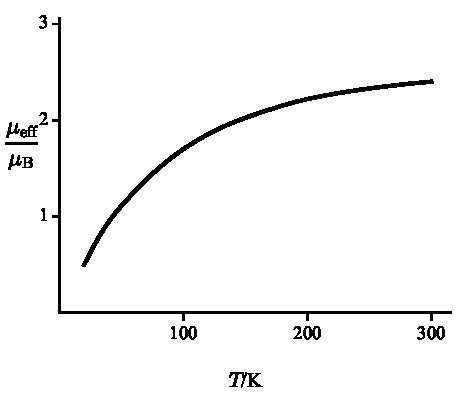
\includegraphics[width=6cm]{fig11-10.pdf}\\{\small 图 11.10\quad 有效杂质磁矩的温度曲线}
\end{minipage}
\end{center}

磁化率反常特征实际上是杂质有效磁矩随温度降低逐渐减小（最后消失）过程在宏观测量上的反映，这是杂质从高温具有确定磁矩 $\mu_{\mathrm{at}}$ 状态向零温度时无磁矩状态的连续变化.由于在s-d模型中是假定杂质具有确定的自旋S，所以 $T=0$ K时所形成的非磁性杂质应当解释为：反铁磁型s-d耦合作用使磁杂质被自旋取向相反的传导电子所包围，从而对杂质磁矩起屏蔽抵消作用，这种抵消倾向随温度降低、热涨落减小而增大，最后在 $T=0$ K时形成一个由杂质和聚集在其周围的反向自旋的传导电子的组合状态，这就是s-d模型中的非磁性杂质态，对应于 $\mu_{\mathrm{eff}}(0)=0$.低温比热容的测量更进一步证实了这种观点.

\subsection*{(ii) 比热容反常}

众所周知，纯金属的低温比热容主要由电子比热容的线性温度律 $\gamma_{\mathrm{e}}T$ 描述.含有一般杂质的金属比热容并不表现出对于线性温度规律的明显偏离，因为这些杂质可以当作是无内结构的外来原子.但是，当金属中含有微量磁性杂质时，比热容将与线性温度规律有严重的偏离，表现为附加在 $\gamma_{\mathrm{e}}T$ 上的一个宽峰曲线，其峰值在低温区，低于电阻极小点.图11.11是CuCr合金的测量曲线.根据热力学，在杂质比热容曲线 $(c_{\text{杂质}}-\ln T)$ 下的面积等于磁杂质在高温和低温时的熵值差
\begin{equation}
\begin{aligned}
  \Delta\mathscr{S}
  &=\int_{0}^{\infty}\frac{c_{\text{杂质}}(T)}{T}\,\mathrm{d}T
  =\mathscr{S}(\infty)-\mathscr{S}(0)\\
  &=k_{\mathrm{B}}\ln(2S+1)
\end{aligned}
\end{equation}
式(11.5.19)中最后一个等式是从实验结果算得的熵差值，其中自旋 $S=3/2$ 正好是Cr在铜中高温测量的自旋值.所以，实验曲线下的面积仅仅等于磁杂质的高温熵值 $k_{\mathrm{B}}\ln(2S+1)$，它要求 $T\to0$ K时磁杂质的熵趋于零，这只能是 $T=0$ K时杂质自旋消失，因为只有这样才能得到零温磁杂质熵
\begin{equation}
  \mathscr{S}(0)=k_{\mathrm{B}}\ln 1=0
\end{equation}
的结果.用s-d模型则解释为零温时（杂质$+$传导电子）系统的总自旋为零.这一总自旋等于零的单重态和磁化率实验所证实的零温度时杂质的非磁特性是一回事，是单个磁杂质与传导电子互作用系统的基态，通常称为近藤单态（Kondo singlet），因为它是非简并的.

\begin{center}
\begin{minipage}{6cm}
\centering
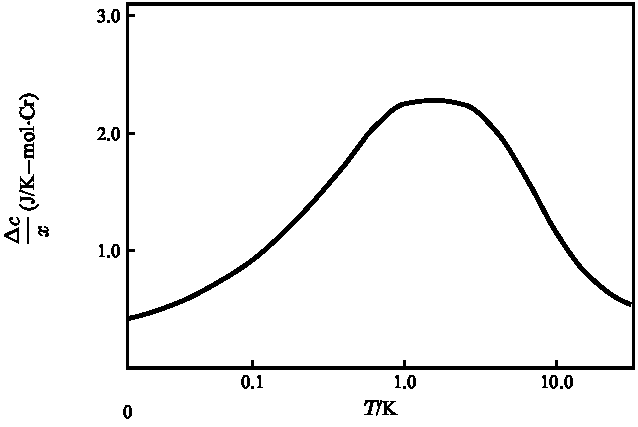
\includegraphics[width=6cm]{fig11-11.pdf}\\{\small 图 11.11\quad CuCr 合金杂质比热容的 ln T 曲线（x 为 Cr 的浓度）}
\end{minipage}
\end{center}

\subsection*{(iii) 低温区的简单平方律}

既然 $T=0$ K时系统的基态是非磁性的近藤单态，与高温时的磁性杂质态完全不同，那么 $T\to0$ K时系统在低温区的特性也应有自己的特征.通过对 $R_{\text{杂质}}$、$\chi_{\text{杂质}}$、$c_{\text{杂质}}$ 的精确实验测量发现，当 $T\to0$ K时它们都与温度T有简单平方的关系：
\begin{equation}
\begin{aligned}
  &R_{\text{杂质}}(T)=R_{\text{杂质}}(0)[1-AT^{2}]\\
  &\chi_{\text{杂质}}(T)=\chi_{\text{杂质}}(0)[1-BT^{2}]\\
  &\frac{(\chi_{\text{杂质}}/\chi_{\mathrm{pauli}})}
  {(c_{\text{杂质}}/c^{\mathrm{e}}_{v})}=2
\end{aligned}
\end{equation}
如图11.12和图11.13所示.由图可知，在 $T\to0$ K时杂质电阻和磁化率的温度曲线都变得平滑化了，这都是由于杂质有效磁矩趋于消失所造成的.例如就杂质电阻而言，在 $T\to0$ K时 $R_{\text{杂质}}$ 趋于饱和，这是因为杂质和周围电子实际上已组成非磁性的近藤单态，从而可以看作是一个"非磁性的外来原子"，它只能提供出与温度几乎无关的剩余电阻，效果与非磁性杂质并无太大差异.

\begin{center}
\begin{minipage}{5cm}
\centering
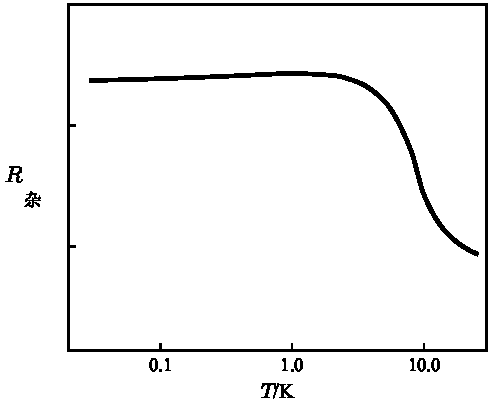
\includegraphics[width=5cm]{fig11-12.pdf}\qquad
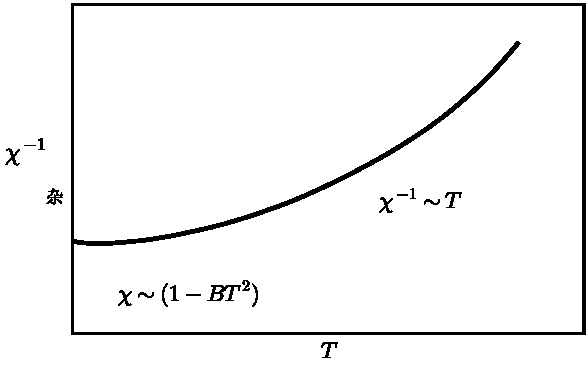
\includegraphics[width=5cm]{fig11-13.pdf}\\[0.3em]
{\small 图 11.12\quad 低温杂质电阻的温度曲线(CuFe 合金)
\qquad 图 11.13\quad 杂质磁化率的温度曲线}
\end{minipage}
\end{center}

综上所述，实验告诉我们近藤效应的本质是金属中单个杂质从磁性状态向非磁性状态的一种连续过渡，在 $T=0$ K时系统的基态是总自旋等于零的单重态.电阻极小，磁化率和比热容的反常等现象都是这一变化在宏观测量上的反映.但是"1"中的微扰计算不适用于低温区，不能用来描述近藤单态.

\subsection*{3. 近藤单态的初步理论}

这里仅介绍芳田奎\textsuperscript{[19]}关于单个磁杂质与传导电子互作用系统的基态理论.他研究 $T=0$ K时一个 $S=1/2$ 的局域自旋与填满的费密球外一个附加电子的s-d耦合系统.把费密球内电子当作自由电子处理，忽略它们可能被杂质散射到球外的复杂情况.因此，费密球的存在仅仅起禁止附加电子占据 $\varepsilon_{k}<0$ 状态的衬底作用.这样做可将近藤哈密顿量（多体哈密顿量）简化为二体问题，与超导理论中的库柏对模型相类似.芳田奎的简化哈密顿量取为
\begin{equation}
  \mathscr{H}_{\mathrm{red}}=\sum_{k,\,\mu}\varepsilon_{k}C^{+}_{k\mu}C_{k\mu}
  -\biggl(\frac{J}{N}\biggr)\sum_{k,\,k'>k_{\mathrm{F}}}\sum_{\mu,\,\mu'}
  \hat{\boldsymbol{S}}\cdot\hat{\boldsymbol{\sigma}}_{\mu\mu'}\,
  C^{+}_{k\mu}C_{k'\mu'}
\end{equation}
与式(11.5.2)相比较可知芳田奎的哈密顿量只考虑了费密球外附加电子与杂质的s-d交换作用.我们可设 $S=1/2$ 局域自旋与传导电子系统的状态为
\begin{equation}
  |\psi\rangle=\sum_{k>k_{\mathrm{F}}}\Gamma_{k}
  \bigl(C^{+}_{k\downarrow}|\uparrow\rangle
  \mp C^{+}_{k\uparrow}|\downarrow\rangle\bigr)|F\rangle
\end{equation}
$|\psi\rangle$ 满足薛定谔方程
\begin{equation}
  (\mathscr{H}_{\mathrm{red}}-E)|\psi\rangle=0
\end{equation}
其中 $|\uparrow\rangle$、$|\downarrow\rangle$ 代表局域自旋朝上及朝下状态，"$-$"代表杂质与附加电子组成的单重态，"$+$"为三重态，包括了芳田奎模型中所有可能组态.$|F\rangle$ 是自由电子的费密球基态，在 $T=0$ K时有
\begin{equation}
\begin{aligned}
  &C^{+}_{k\mu}|F\rangle=0\quad(\text{当}\ \varepsilon_{k}<0\ \text{时})\\
  &C_{k\mu}|F\rangle=0\quad(\text{当}\ \varepsilon_{k}>0\ \text{时})
\end{aligned}
\end{equation}
费密球态的哈密顿量为
\begin{equation}
  \mathscr{H}^{\mathrm{F}}_{0}
  =\sum_{k<k_{\mathrm{F}}}\sum_{\mu}\varepsilon_{k}C^{+}_{k\mu}C_{k\mu}
\end{equation}
相应的能量设为 $E_{\mathrm{g}}$，它满足方程
$(\mathscr{H}^{\mathrm{F}}_{0}-E_{\mathrm{g}})|F\rangle=0$.
显然，$|\psi\rangle$ 也满足方程
\begin{equation}
  (\mathscr{H}^{\mathrm{F}}_{0}-E_{\mathrm{g}})|\psi\rangle=0
\end{equation}
式(11.5.24)与式(11.5.27)相减得
\begin{equation}
  (\overline{\mathscr{H}}-\overline{E})|\psi\rangle=0
\end{equation}
这里
\begin{equation}
  \overline{\mathscr{H}}
  =\sum_{k>k_{\mathrm{F}}}\sum_{\mu}\varepsilon_{k}C^{+}_{k\mu}C_{k\mu}
  -\frac{J}{N}\sum_{k,\,k'>k_{\mathrm{F}}}\sum_{\mu,\,\mu'}
  \hat{\boldsymbol{S}}\cdot\hat{\boldsymbol{\sigma}}_{\mu\mu'}\,
  C^{+}_{k\mu}C_{k'\mu'}
\end{equation}
只涉及费密球外问题，而
\begin{equation}
  \overline{E}=E-E_{\mathrm{g}}
\end{equation}
代表局域自旋与费密球外附加电子的束缚能.用共轭态向量
\begin{equation*}
  \langle F|\bigl(C_{k\downarrow}\langle\uparrow|
  \mp C_{k\uparrow}\langle\downarrow|\bigr)
\end{equation*}
左乘式(11.5.28)，并利用对易式
\begin{equation}
\begin{aligned}
  &[C^{+}_{k\mu},C_{k'\mu'}]_{+}=\delta_{kk'}\delta_{\mu\mu'}\\
  &[C^{+}_{k\mu},C^{+}_{k'\mu'}]_{+}
  =[C_{k\mu},C_{k'\mu'}]_{+}=0
\end{aligned}
\end{equation}
和局域自旋关系
\begin{equation}
\begin{aligned}
  &\hat{S}^{\pm}|\uparrow\rangle
  =\begin{cases}0&(+)\smallskip\\|\downarrow\rangle&(-)\end{cases}\\
  &\hat{S}^{\pm}|\downarrow\rangle
  =\begin{cases}|\uparrow\rangle&(+)\smallskip\\0&(-)\end{cases}\\
  &\hat{S}^{z}|\alpha\rangle=\pm\frac{1}{2}|\alpha\rangle
  \qquad\alpha=\begin{cases}\uparrow\\\downarrow\end{cases}
\end{aligned}
\end{equation}
容易算得对于单重态 $\Gamma_{k}$ 满足方程
\begin{equation}
  2(\varepsilon_{k}-\overline{E})\Gamma_{k}
  +\frac{3J}{N}\sum_{k'>k_{\mathrm{F}}}\Gamma_{k'}=0
\end{equation}
对于三重态，$\Gamma_{k}$ 的方程为
\begin{equation}
  2(\varepsilon_{k}-\overline{E})\Gamma_{k}
  -\frac{J}{N}\sum_{k'>k_{\mathrm{F}}}\Gamma_{k'}=0
\end{equation}
与库柏对问题相似，用 $2(\varepsilon_{k}-\overline{E})$ 除式(11.5.33)和式(11.5.34)，并对k求和.考虑到 $\Gamma_{k}$ 有非零解存在，因此可利用关系
\begin{equation}
  \sum_{k>k_{\mathrm{F}}}\Gamma_{k}=\text{常数}
\end{equation}
消去 $\Gamma_{k}$.对于单重态得到
\begin{equation}
  1+\frac{3J}{2N}\sum_{k>k_{\mathrm{F}}}
  \frac{1}{\varepsilon_{k}-\overline{E}}=0
\end{equation}
而三重态则为
\begin{equation}
  1-\frac{J}{2N}\sum_{k>k_{\mathrm{F}}}
  \frac{1}{\varepsilon_{k}-\overline{E}}=0
\end{equation}
采用简化态密度式(11.5.13)计算求和
\begin{equation}
\begin{aligned}
  \frac{J}{N}\sum_{k>k_{\mathrm{F}}}\frac{1}{\varepsilon_{k}-\overline{E}}
  &\approx J\rho_{\mathrm{F}}\int_{0}^{D}
  \frac{\mathrm{d}\varepsilon}{\varepsilon-\overline{E}}\\
  &=J\rho_{\mathrm{F}}\ln\biggl[\frac{\overline{E}-D}{\overline{E}}\biggr]
\end{aligned}
\end{equation}
当 $|J|\rho_{\mathrm{F}}\ll1$ 时，求得对于反铁磁型s-d耦合 $(J<0)$ 单重态的束缚能为
\begin{equation}
  \overline{E}_{\mathrm{s}}\approx
  -D\exp\biggl[-\frac{2}{3|J|\rho_{\mathrm{F}}}\biggr]
  \qquad(J<0)
\end{equation}
而三重态 $E_{\mathrm{t}}\approx D$ 是不稳定的.只有当 $J>0$ 时三重态才是稳定的
\begin{equation}
  \overline{E}_{\mathrm{t}}\approx
  -D\exp\biggl[-\frac{2}{|J|\rho_{\mathrm{F}}}\biggr]
  \qquad(J>0)
\end{equation}
这时单重态不稳定.

由于近藤效应只是 $J<0$ 时稀磁合金的特征，因此芳田奎的理论告诉我们系统的基态是近藤单态，与实验结果一致.

芳田奎的基态理论忽略了与费密球内电子的相互作用，显然过于粗糙.事实上在低温区近藤问题是很复杂的，由于杂质原子本身具有内自由度（自旋的 $2S+1$ 个取向），当第一个电子通过s-d互作用被散射后，杂质自旋取向要发生变化，这种自旋状态的改变又将直接影响第二个电子在此杂质上的散射，因此相继在杂质上被散射的电子之间存在着通过杂质的间接相互作用，这是一种关联效应.随着温度降低，热涨落减小，关联效应将越来越强，以至在很低温度时任何一个电子的散射都将和系统中所有其它 $(N-1)$ 个电子的运动状态牵连在一起，这里涉及到必须同时考虑所有粒子相互作用的真正多体问题.这一困难直到20世纪70年代在统计力学发展的基础上才得到真正解决，1975年，威尔逊（K.G.Wilson）\textsuperscript{[20]}用实空间重正化群方法严格证明了 $T=0$ K时系统的基态是近藤单态，推广于 $T\neq0$ K情况所计算的磁化率曲线在全温区也与实验一致.威尔逊解只是数值解，1980年，美国\textsuperscript{[21]}和（前）苏联学者\textsuperscript{[22]}应用贝脱方案（Bethe ansatz）又求得了单杂质近藤问题的严格解析解，至此问题才算解决.

最后，还应指出在单杂质的近藤问题中存在一个特征温度 $T_{\mathrm{K}}$，称 $T_{\mathrm{K}}$ 为近藤温度，它是大致划分系统从高温 $(T\gg T_{\mathrm{K}})$ 磁矩态向低温 $(T\ll T_{\mathrm{K}})$ 非磁态渡越的特征温度.当 $T\gg T_{\mathrm{K}}$ 时磁杂质满足居里-外斯定律，其杂质电阻由式(11.5.16)描述，表现为独立磁离子特性，而当 $T\ll T_{\mathrm{K}}$ 时，由于多体关联，局域磁矩将被传导电子屏蔽，形成非磁性的近藤单态，而 $k_{\mathrm{B}}T_{\mathrm{K}}$ 则定义为零温时形成单态系统所降低的能量 $(-\overline{E}_{\mathrm{s}})$.芳田奎等人经过努力，成功地计入了含无穷个电子-空穴对激发的主导项，求得的 $\overline{E}_{\mathrm{s}}$ 相当于将式(11.5.39)的指数中(2/3)因子用(1/2)代替，这时
\begin{equation}
  k_{\mathrm{B}}T_{\mathrm{K}}\equiv-\overline{E}_{\mathrm{s}}
  =D\exp\biggl[-\frac{1}{2\rho_{\mathrm{F}}|J|}\biggr]
\end{equation}
其中D为导带的半宽度，而费密面上传导电子的态密度取为
\begin{equation}
  \rho_{\mathrm{F}}=1/2D
\end{equation}
详细的讨论可参阅修森（Hewson）的专著（文献[24]）.

\section{施里弗-沃尔夫变换}

讲的是如何从安德逊模型导出s-d交换模型.在历史上是施里弗和沃尔夫（Wolff）\textsuperscript{[23]}采用类似于式(5.5.8)—式(5.5.11)的正则变换方法消去安德逊模型中s-d混合作用［式(11.2.4)］的一阶项，首先导出了描述近藤效应的s-d交换模型.因此，人们就将上述两个模型之间的转换关系称为施里弗-沃尔夫变换.在本节中我们将采用投影算符技巧\textsuperscript{[24]}作推导，这样做在物理图像上更为清楚.

从轨道非简并的安德逊模型式(11.2.5)出发，在无外磁场和略去s-d混合作用强度对k的依赖（即取 $V_{kd}=V$）条件下，将哈密顿量写为
\begin{equation}
  H=\sum_{k,\,\sigma}E_{k}C^{+}_{k\sigma}C_{k\sigma}
  +\sum_{\sigma}E_{\mathrm{d}}n_{\mathrm{d}\sigma}
  +Un_{\mathrm{d}\uparrow}n_{\mathrm{d}\downarrow}
  +H_{\mathrm{mix}}
\end{equation}
其中
\begin{equation}
  H_{\mathrm{mix}}=V\sum_{k,\,\sigma}
  \bigl(d^{+}_{\sigma}C_{k\sigma}+C^{+}_{k\sigma}d_{\sigma}\bigr)
\end{equation}
\begin{equation}
  n_{\mathrm{d}\sigma}=d^{+}_{\sigma}d_{\sigma}
\end{equation}
注意到安德逊模型在 $V=0$ 时，由于局域的d电子不与传导电子相耦合，杂质的两个d轨道能级分别为 $E_{\mathrm{d}}$ 与 $E_{\mathrm{d}}+U$.这时系统存在3种不同的d电子组态：(i)两个d能级均为零占据，对应的总能量为 $E_{0}=0$；(ii)自旋 $\sigma$ 的单占据组态，总能量为 $E_{1\sigma}=E_{\mathrm{d}}$，其中 $\sigma=\uparrow$ 或 $\downarrow$；(iii)双占据组态，两个能级分别被一个自旋 $\uparrow$ 和一个自旋 $\downarrow$ 的电子所占据，对应的总能量为 $2E_{\mathrm{d}}+U$，如图11.14所示.

\begin{center}
\begin{minipage}{9cm}
\centering
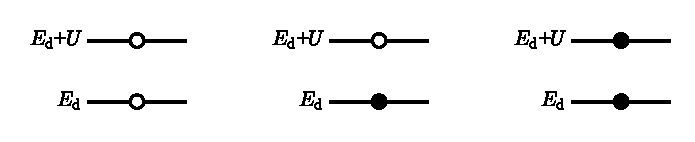
\includegraphics[width=9cm]{fig11-14.pdf}\\[0.3em]
{\small (a) 零占据\qquad\qquad (b) 单占据\qquad\qquad (c) 双占据}\\[0.2em]
{\small 图 11.14\quad 杂质上的 d 电子组态}
\end{minipage}
\end{center}

如果基态对应于单占据组态，则要求 $E_{\mathrm{d}}<E_{\mathrm{F}}$ 和 $E_{\mathrm{d}}+U>E_{\mathrm{F}}$，若再取传导电子的费密能级 $E_{\mathrm{F}}$ 为能量的原点，则只有单占据组态的总能量小于零，而双占据与零占据组态的总能量将大于或等于零.这时杂质的基态将是存在一个自旋 $\uparrow$ 或 $\downarrow$ 的有局域矩的磁性状态，而激发态则对应于零占据或双占据的无局域磁矩状态.我们的问题是要研究当局域d态与传导电子之间存在混合作用（即 $V\neq0$）时安德逊模型中的局域磁矩特征.我们将证明，当V足够弱时安德逊模型可直接简化为§3中的s-d交换模型.

在一般情况下，可以将安德逊模型在希尔伯特空间划分为3个子空间，并相应地引入3套投影算符
\begin{equation}
\begin{aligned}
  &P_{0}=(1-n_{\mathrm{d}\uparrow})(1-n_{\mathrm{d}\downarrow})\\
  &P_{1}=n_{\mathrm{d}\uparrow}(1-n_{\mathrm{d}\downarrow})
  +n_{\mathrm{d}\downarrow}(1-n_{\mathrm{d}\uparrow})\\
  &P_{2}=n_{\mathrm{d}\uparrow}n_{\mathrm{d}\downarrow}
\end{aligned}
\end{equation}
其中 $P_{n}$ 代表投影到占据数 $n=0,\,1,\,2$ 的空占据，单占据和双占据子空间的算符，并且满足投影算符的基本规则：
\begin{equation*}
\begin{aligned}
  &P^{2}_{n}=P_{n}\qquad(n=0,\,1,\,2)\\
  &P_{0}P_{1}=P_{1}P_{2}=P_{0}P_{2}=0
\end{aligned}
\end{equation*}
相应地在全希尔伯特空间中，系统的总波函数 $\varPsi$ 可由3个子空间中的分量 $\psi_{0}$、$\psi_{1}$ 和 $\psi_{2}$ 作线性组合构成，这时薛定谔方程 $H\varPsi=E\varPsi$ 可以表示为
\begin{equation}
  \begin{pmatrix}
    H_{00}&H_{01}&H_{02}\\
    H_{10}&H_{11}&H_{12}\\
    H_{20}&H_{21}&H_{22}
  \end{pmatrix}
  \begin{pmatrix}\psi_{0}\\\psi_{1}\\\psi_{2}\end{pmatrix}
  =E\begin{pmatrix}\psi_{0}\\\psi_{1}\\\psi_{2}\end{pmatrix}
\end{equation}
其中 $H_{nn'}=P_{n}HP_{n'}$.对于安德逊模型，由于不存在同时产生和消灭两个d电子的互作用，所以 $H_{02}=H_{20}=0$，其它的非对角矩阵元如 $H_{01}$ 和 $H_{12}$ 均来自 $H_{\mathrm{mix}}$.运用泡利原理和费密子的算符等式 $n^{2}_{\mathrm{d}\sigma}=n_{\mathrm{d}\sigma}$ 可导出

\begin{subequations}
\begin{equation}
  H_{01}=P_{0}HP_{1}=P_{0}H_{\mathrm{mix}}P_{1}
  =V\sum_{k,\,\sigma}C^{+}_{k\sigma}
  \bigl(1-n_{\mathrm{d}\bar{\sigma}}\bigr)d_{\sigma}
\end{equation}
\begin{equation}
  H_{12}=P_{1}HP_{2}=P_{1}H_{\mathrm{mix}}P_{2}
  =V\sum_{k,\,\sigma}C^{+}_{k\sigma}d_{\sigma}n_{\mathrm{d}\bar{\sigma}}
\end{equation}
\end{subequations}

并且矩阵是厄米的，有 $H_{10}=H^{+}_{01}$ 与 $H_{21}=H^{+}_{12}$ 关系.

现在讨论存在 $H_{\mathrm{mix}}$ 项时的d轨道单占据解.为此，从式(11.6.5)中消去 $\psi_{0}$ 和 $\psi_{2}$ 态，求得在单占据子空间的一个等效方程
\begin{equation}
  \widetilde{H}\psi_{1}=E_{1}\psi_{1}
\end{equation}
其中
\begin{equation}
  \widetilde{H}=H_{11}
  +H_{12}(E-H_{22})^{-1}H_{21}
  +H_{10}(E-H_{00})^{-1}H_{01}
\end{equation}
代表单占据子空间中的有效哈密顿量.到此为止，我们尚未作任何近似，式(11.6.8)仍是严格的.施里弗-沃尔夫变换则只是在准至V二阶的微扰范围内计入系统从单占据向零占据和双占据等状态的虚激发，这时 $(E-H_{22})$ 可近似用 $V=0$ 时单占与双占态的能量差 $(E_{k'}-E_{\mathrm{d}}-U)$ 代替，它表示传导电子 $E_{k'}$ 进入杂质d轨道的高能级 $E_{\mathrm{d}}+U$.类似的，对于 $(E-H_{00})$ 也可用 $(E_{\mathrm{d}}-E_{k})$ 代替，表明单占据的 $E_{\mathrm{d}}$ 电子逸出d轨道成为传导电子 $E_{k}$.再运用式(11.6.6)，在准至V二阶条件下，可将式(11.6.8)中的两个虚激项分别写为

\begin{subequations}
\begin{equation}
\begin{aligned}
  H_{12}(E-H_{22})^{-1}H_{21}
  &=\sum_{k,\,k',\,\sigma,\,\sigma'}
  \frac{V^{2}}{(U+E_{\mathrm{d}}-E_{k'})}(-1)\\
  &\qquad\times C^{+}_{k\sigma}C_{k'\sigma'}d_{\sigma}
  n_{\mathrm{d}\bar{\sigma}}d^{+}_{\sigma'}n_{\mathrm{d}\bar{\sigma}'}
\end{aligned}
\end{equation}
\begin{equation}
\begin{aligned}
  H_{10}(E-H_{00})^{-1}H_{01}
  &=\sum_{k,\,k',\,\sigma,\,\sigma'}
  \frac{V^{2}}{(E_{\mathrm{d}}-E_{k})}(-1)
  C^{+}_{k\sigma}C_{k'\sigma'}d^{+}_{\sigma'}
  \bigl(1-n_{\mathrm{d}\bar{\sigma}'}\bigr)\\
  &\qquad\times d_{\sigma}\bigl(1-n_{\mathrm{d}\bar{\sigma}'}\bigr)
\end{aligned}
\end{equation}
\end{subequations}

在满足单占据条件 $n_{\mathrm{d}}=n_{\mathrm{d}\uparrow}+n_{\mathrm{d}\downarrow}=1$ 时，根据自旋 $\dfrac{1}{2}$ 的算符等式：
\begin{equation}
\left.
\begin{aligned}
  &\hat{S}^{z}=\frac{1}{2}
  (d^{\dagger}_{\uparrow}d_{\uparrow}
  -d^{\dagger}_{\downarrow}d_{\downarrow})\\
  &\hat{S}^{+}=d^{\dagger}_{\uparrow}d_{\downarrow}\\
  &\hat{S}^{-}=d^{\dagger}_{\downarrow}d_{\uparrow}
\end{aligned}\right\}
\end{equation}
经简单运算，可将式(11.6.9a)中算符归并为如下3种类型：
\begin{equation*}
\begin{aligned}
  &\text{(i)}\ \sigma=\downarrow\ \text{与}\ \sigma'=\uparrow\ \text{项：}
  \ C^{+}_{k\downarrow}C_{k'\uparrow}d^{\dagger}_{\uparrow}d_{\downarrow}
  =\hat{S}^{+}C^{+}_{k\downarrow}C_{k'\uparrow}\\
  &\text{(ii)}\ \sigma=\uparrow\ \text{与}\ \sigma'=\downarrow\ \text{项：}
  \ C^{+}_{k\uparrow}C_{k'\downarrow}d^{\dagger}_{\downarrow}d_{\uparrow}
  =\hat{S}^{-}C^{+}_{k\uparrow}C_{k'\downarrow}\\
  &\text{(iii)}\ \sigma=\sigma'=\uparrow\ \text{和}\ \sigma=\sigma'=\downarrow\ \text{项：}
  \ \hat{S}^{z}\bigl(C^{+}_{k\uparrow}C_{k'\uparrow}
  -C^{+}_{k\downarrow}C_{k'\downarrow}\bigr)\\
  &\hphantom{\text{(iii)}\ \sigma=\sigma'=\uparrow\ \text{和}\ \sigma=\sigma'=\downarrow\ \text{项：}\ \hat{S}^{z}(\cdots)\ }
  -\frac{1}{2}\sum_{\sigma}C^{+}_{k\sigma}C_{k'\sigma}
\end{aligned}
\end{equation*}
由此求得
\begin{equation}
\begin{aligned}
  H_{12}(E-H_{22})^{-1}H_{21}
  &=\sum_{k,\,k'}\frac{V^{2}}{(U+E_{\mathrm{d}}-E_{k'})}
  \bigl\{\bigl[\hat{S}^{z}\bigl(C^{+}_{k\uparrow}C_{k'\uparrow}
  -C^{+}_{k\downarrow}C_{k'\downarrow}\bigr)\\
  &\qquad+\hat{S}^{+}C^{+}_{k\downarrow}C_{k'\uparrow}
  +\hat{S}^{-}C^{+}_{k\uparrow}C_{k'\downarrow}\bigr]
  -\frac{1}{2}\sum_{\sigma}C^{+}_{k\sigma}C_{k'\sigma}\bigr\}
\end{aligned}
\end{equation}
类似的讨论可证明
\begin{equation}
\begin{aligned}
  H_{10}(E-H_{00})^{-1}H_{01}
  &=\sum_{k,\,k'}\frac{V^{2}}{(E_{k}-E_{\mathrm{d}})}
  \bigl\{\bigl[\hat{S}^{z}\bigl(C^{+}_{k\uparrow}C_{k'\uparrow}
  -C^{+}_{k\downarrow}C_{k'\downarrow}\bigr)\\
  &\qquad+\hat{S}^{+}C^{+}_{k\downarrow}C_{k'\uparrow}
  +\hat{S}^{-}C^{+}_{k\uparrow}C_{k'\downarrow}\bigr]
  +\frac{1}{2}\sum_{\sigma}C^{+}_{k\sigma}C_{k'\sigma}\bigr\}
\end{aligned}
\end{equation}
再考虑到略去常数项 $E_{\mathrm{d}}$ 后，$H_{11}$ 简化为传导电子的自由项
\begin{equation}
  H_{o}=\sum_{k,\,\sigma}E_{k}C^{+}_{k\sigma}C_{k\sigma}
\end{equation}
将上述结果代入式(11.6.8)，求得在单占据子空间中的有效哈密顿量
\begin{equation}
  \widetilde{H}=H_{o}+H_{\mathrm{p}}+H_{\mathrm{sd}}
\end{equation}
其中 $H_{\mathrm{p}}$ 只是一般的杂质势散射项
\begin{equation}
  H_{\mathrm{p}}=\sum_{k,\,k',\,\sigma}\frac{V^{2}}{2}
  \biggl\{\frac{1}{(E_{k}-E_{\mathrm{d}})}
  -\frac{1}{(U+E_{\mathrm{d}}-E_{k'})}\biggr\}
  C^{+}_{k\sigma}C_{k'\sigma}
\end{equation}
而 $H_{\mathrm{sd}}$ 则代表与杂质的自旋自由度有关的s-d交换作用项
\begin{equation}
  H_{\mathrm{sd}}=-\sum_{k,\,k'}J_{kk'}
  \bigl\{\hat{S}^{z}\bigl(C^{+}_{k\uparrow}C_{k'\uparrow}
  -C^{+}_{k\downarrow}C_{k'\downarrow}\bigr)
  +\hat{S}^{+}C^{+}_{k\downarrow}C_{k'\uparrow}
  +\hat{S}^{-}C^{+}_{k\uparrow}C_{k'\downarrow}\bigr\}
\end{equation}
其耦合强度为
\begin{equation}
  J_{kk'}=-V^{2}\biggl\{\frac{1}{(E_{k}-E_{\mathrm{d}})}
  +\frac{1}{(U+E_{\mathrm{d}}-E_{k'})}\biggr\}
\end{equation}
由于与杂质自旋相互作用的传导电子均位于费密面附近，人们可以将上式中的 $E_{k}$ 与 $E_{k'}$ 近似取为 $E_{\mathrm{F}}$，再考虑到在局域矩区域有 $U+E_{\mathrm{d}}>E_{\mathrm{F}}>E_{\mathrm{d}}$ 条件，因此 $J_{kk'}<0$，说明在杂质自旋与传导电子自旋之间的耦合是反铁磁型s-d耦合，它导致近藤效应.在强关联极限下可取 $U\to\infty$，这时s-d交换作用简化为与k及 $k'$ 均无关的耦合常数
\begin{equation}
  J_{kk'}=J=-\frac{V^{2}}{|E_{\mathrm{d}}-E_{\mathrm{F}}|}<0
\end{equation}
这时若略去杂质的一般性势散射效应，$\widetilde{H}$ 将直接写成
\begin{equation}
\begin{aligned}
  \widetilde{H}&=\sum_{k,\,\sigma}E_{k}C^{+}_{k\sigma}C_{k\sigma}
  -J\sum_{k,\,k'}\bigl\{\hat{S}^{z}\bigl(C^{+}_{k\uparrow}C_{k'\uparrow}
  -C^{+}_{k\downarrow}C_{k'\downarrow}\bigr)\\
  &\qquad+\hat{S}^{+}C^{+}_{k\downarrow}C_{k'\uparrow}
  +\hat{S}^{-}C^{+}_{k\uparrow}C_{k'\downarrow}\bigr\}
\end{aligned}
\end{equation}
与描述近藤效应的哈密顿量式(11.5.2)相同.差别仅在于那里的 $(J/N)$ 对应于上式中的J.

综上所述，从单杂质安德逊模型出发，在传导电子与局域电子之间的混合作用V很弱时，研究系统从单占据基态 d$^{1}$ 向零占据态 d$^{0}$ 和双占据态 d$^{2}$ 等激发态的虚跃迁效应，在准至V的二阶近似下证明了这类激发等效于s-d交换作用.因此，人们常说当V很小时安德逊模型可直接过渡到描述近藤效应的s-d交换模型.从物理上讲，s-d交换模型是在d电子满足单占据条件下导出的，在那里d电子的电荷涨落（即杂质的价涨落）效应已被忽略，但是，在安德逊模型中由于存在混合作用V，局域电子与传导电子之间有相互转移，将导致局域电子的电荷涨落（或杂质的价涨落）效应.因此，这两个模型是有区别的，并且后者涉及更为广泛的物理问题.仅当V足够的弱，d$^{0}$ 与 d$^{2}$ 等组态相对于单占据组态 d$^{1}$ 的占据比例小到可以忽略时，安德逊模型才能够用一个不计电荷涨落的s-d交换模型来代替.换句话说，施里弗-沃尔夫变换正是在混合作用十分微弱的条件下，消去V所产生的电荷涨落，代之以一个局域自旋与传导电子自旋的非直接交换作用，使安德逊模型过渡为s-d交换模型，被称为安德逊模型的近藤极限.在此极限下，杂质的电荷涨落被压制，表现为局域自旋矩特征，它与传导电子间的耦合仅产生自旋的取向变化，导致系统的自旋涨落.

安德逊模型存在两个有意义的极限，它们是近藤极限和变价（又称混合价）极限.近藤极限首先要求杂质处于局域矩状态.当 $V=0$ 时，存在局域矩（或单占据基态）的条件已给出为 $E_{\mathrm{d}}<E_{\mathrm{F}}$ 与 $E_{\mathrm{d}}+U>E_{\mathrm{F}}$，物理上对应于要求费密能级位于两个自旋劈裂能级之间.当计入混合作用V之后，系统形成局域矩的条件可近似由外场 $h=0$ 时的自洽方程式(11.2.33)决定，它们是
\begin{equation}
\left.
\begin{aligned}
  \langle n_{\mathrm{d}\uparrow}\rangle
  &=\frac{1}{\pi}\mathrm{arccot}
  \biggl[\frac{E_{\mathrm{d}}-E_{\mathrm{F}}
  +U\langle n_{\mathrm{d}\downarrow}\rangle}{\Gamma}\biggr]\\
  \langle n_{\mathrm{d}\downarrow}\rangle
  &=\frac{1}{\pi}\mathrm{arccot}
  \biggl[\frac{E_{\mathrm{d}}-E_{\mathrm{F}}
  +U\langle n_{\mathrm{d}\uparrow}\rangle}{\Gamma}\biggr]
\end{aligned}\right\}
\end{equation}
其中 $\Gamma=\pi V^{2}\rho^{(0)}(E_{\mathrm{F}})$ 代表杂质d轨的共振线半宽度.显然，当满足下列条件时
\begin{equation}
\begin{gathered}
  E_{\mathrm{d}}<E_{\mathrm{F}},
  \quad E_{\mathrm{d}}+U>E_{\mathrm{F}}\\
  \text{和}\\
  |E_{\mathrm{d}}+U-E_{\mathrm{F}}|,\ |E_{\mathrm{d}}-E_{\mathrm{F}}|\gg\Gamma
\end{gathered}
\end{equation}
存在 $\langle n_{\mathrm{d}\uparrow}\rangle\to1$，$\langle n_{\mathrm{d}\downarrow}\rangle\to0$ 的局域矩解，这时磁杂质的平均电子数并无显著变化，仍保持整数价.应当指出，式(11.6.21)中包含了形成局域磁矩的最有利条件 $\Gamma\ll U$.正是在此强关联与弱杂化条件下，杂质的电荷涨落被压制，安德逊模型才能演化为描述局域自旋矩与传导电子自旋之间的反铁磁型交换作用的s-d交换模型，并用于解释近藤效应.因此，式(11.6.21)是近藤极限（又称整数价极限）的参数条件.在具体运用安德逊模型讨论金属中的过渡和稀土磁性杂质时，人们往往直接从强关联极限 $(U\to\infty)$ 情形出发，由于在 $E_{\mathrm{d}}+U$ 能级上不可能占据电子，近藤极限条件简化为要求 $(E_{\mathrm{d}}-E_{\mathrm{F}})$ 取大的负值，即 $|E_{\mathrm{d}}-E_{\mathrm{F}}|\gg\Gamma$，并可求出一个与k无关的s-d交换作用 $J=-V^{2}/|E_{\mathrm{d}}-E_{\mathrm{F}}|$.安德逊模型的另一个极限出现在 $E_{\mathrm{d}}$ 能级比较接近 $E_{\mathrm{F}}$ 以至 $|E_{\mathrm{d}}-E_{\mathrm{F}}|$ 与 $\Gamma$ 值相近的情形，这时杂质的电荷涨落变得十分重要，在杂质的局域轨道态与传导电子的费密海之间将出现电荷的实际转移，它们不能再用二级微扰的虚激发过程处理，因此施里弗-沃尔夫变换失效，人们必须从 $U=\infty$ 的安德逊模型出发来讨论这一极限情形.由于电荷涨落，磁性杂质不再具有整数价，而是两种或多种价态的混合，这种具有非整数价特征情形被称之为变价极限.典型的例子是高压下的稀土化合物SmS，电荷涨落使Sm$^{2+}$离子有一定概率变为Sm$^{3+}$，使Sm离子处于介乎2价与3价之间的中间价态 Sm$^{\nu+}$（$\nu=2.75$），这类材料也相应地称之为价变（或中间价）化合物.显然，$U=\infty$ 的安德逊模型是讨论金属中磁杂质近藤效应和变价特性的一个良好理论模型，在此模型中，若取 $E_{\mathrm{d}}$ 远远低于 $E_{\mathrm{F}}$，将得到近藤极限，而取 $E_{\mathrm{d}}$ 十分靠近 $E_{\mathrm{F}}$ 又可达变价极限.

近年来，在含有未填满的f壳层稀土（如Ce、4f）及锕系（如U、5f）元素的多元化合物中发现了新的一类固体材料，其中大多数材料具有金属性，其共同的特点是低激发态具有很高的电子有效质量 $(m^{*}/m_{\mathrm{e}}\gg1)$，被称为重电子金属，理论上属于重费密子系统.在重费密子系统中已发现了3种不同的金属型基态.它们是：重费密子超导体（CeCu$_{2}$Si$_{2}$、UBe$_{13}$、UPt$_{3}$等），重费密子磁体（U$_{2}$Zn$_{17}$、UCd$_{11}$、NpBe$_{13}$等）和重费密子液体（CeAl$_{3}$、CeCu$_{6}$、YbCuAl等）.这些材料的零温电子比热容的线性温度系数 $\gamma$ 可高达 $100\sim1000$ mJ/(mol$\cdot$K$^{2}$)，比普通金属的 $\gamma$ 值 $1\sim10$ mJ/(mol$\cdot$K$^{2}$)平均高100倍，最高可达1000倍.由于 $\gamma\sim m^{*}$，而在普通金属中 $m^{*}$ 与自由电子质量 $m_{\mathrm{e}}$ 同量级，因此近期对重费密子系统有效质量的下界大致规定在 $m^{*}\geqslant10\sim100\,m_{\mathrm{e}}$ 的较宽松区域内\textsuperscript{[25]}.这样做可统一概括早期对重费密子系统的"轻量级" $(m^{*}/m_{\mathrm{e}}>10)$、"中等量级" $(m^{*}/m_{\mathrm{e}}>50)$ 以及"重量级" $(m^{*}/m_{\mathrm{e}}>100)$ 等繁琐分类.20世纪90年代以来在4f族化合物（Ce$_{3}$Bi$_{4}$Pt$_{3}$、CeRhSb、CeNiSn）中发现了具有绝缘性基态的重费密子材料，加上早期的绝缘性化合物SmB$_{6}$和YbB$_{12}$构成重费密子系统中新一类，它们具有不同寻常的小能隙 $(\Delta=1\sim10$ meV，对应于 $10\sim100$ K$)$ 半导体特征，称为重费密子半导体或近藤绝缘体，其能隙是温度的函数，并且对掺杂、加压和外磁场均十分敏感，在Ce$_{3}$Bi$_{4}$Pt$_{3}$中，当温度T上升到接近零温 $\Delta$ 值时，或用La替代Ce作掺杂 (La$_{x}$Ce$_{1-x}$)$_{3}$Bi$_{4}$Pt$_{3}$，均可能使能隙消失，这时近藤绝缘体系统过渡为重费密子金属，并具有高的比热容系数，例如 $x=0.3$ 时 $\gamma$ 可高达150 mJ/(mol$\cdot$K$^{2}$)，应属重费密子系统.

从理论上讲，重费密子系统是每个元胞中均含有稀土和锕系离子的晶格系统.高温磁化率测量表明，无论是重费密子金属或半导体均表现为如同独立磁性离子那样满足居里-外斯规律，说明f电子在强关联 $U\gg\Gamma$ 条件下形成了局域磁矩，与金属中含单个磁杂质的近藤问题有相似之处，差别仅在于重费密子材料是近藤离子呈周期性排列的晶格系统，人们称之为近藤晶格系统.由于安德逊模型是描述单杂质近藤问题的良好出发点，人们普遍相信，若将它作周期性推广，构成安德逊晶格模型也将是描述重费密子系统（或近藤晶格）本质特征的一个基本模型.类似于单杂质近藤问题，重费密子系统与近藤晶格也属于 $U\gg\Gamma$ 的强关联电子体系，在具体进行理论处理时，可采用 $U=\infty$ 的安德逊晶格模型.但应注意，在强关联情况下在本章§2中对同格点库仑关联作平均场近似的方案失效，必须寻找处理强关联系统的良好近似，其中之一就是下节中将介绍的隶玻色技巧的平均场近似.
